\documentclass[]{thesis}  % draft mode (default)
% \documentclass[review]{thesis}  % review mode (show contents & reference only)
% \documentclass[watermark,final]{thesis}  % final mode (version for library)

%-------------------------------------------------------------------------------
% Package Loading
%-------------------------------------------------------------------------------

\usepackage{multirow}     % for multi-row table
\usepackage{booktabs}     % table style used in books

%-------------------------------------------------------------------------------
% Configuration
%-------------------------------------------------------------------------------

% 填寫題目, 作者, 指導教授, 學校, 系所, 日期等資訊
% Title
\title{Unseen defect image synthesis with compositional conditional diffusion model}
\titlezh{基於條件擴散模型的未見缺陷圖像合成 }

% Author
\author{Pin-Chuan Chen}
\authorzh{陳品銓}

% Advisor
\advisor{Ching-Wen Ma}
\advisorzh{馬清文}

% First co-advisor (Leave {} empty if you don't have a co-advisor)
\coadvisorA{}
\coadvisorAzh{}

% Second co-advisor (Leave {} empty if you don't have a second co-advisor)
\coadvisorB{}
\coadvisorBzh{}

% Field
\field{Artificial Intelligence}

% Institute
\institute{Institute of Computational  Intelligence}
\institutezh{智慧計算與科技研究所}

% College
\college{College of Artificial Intelligence}

% University
\university{National Yang Ming Chiao Tung University}
\universityzh{國立陽明交通大學}

% Location
\location{Taiwan, Republic of China}

% Date of final submission
\degreemonth{May}
\degreeyear{2024}
\degreeyearzh{中華民國 一一三年五月}

% Date of final submission
\nation{中華民國}
\yearmonth{一一三年五月}

% Watermark %At present(v.1 2021.Sep.29, v.2 2022.Feb.25), not water wark for NYCU yet.
% \watermark{figures/nycu_logo_1.png}

% 修改 thesis.cls 的預設字型
%-------------------------------------------------------------------------------
% Chinese Font Settings
%
%   These macros are used to change the default Chinese fonts (see below) used
% by thesis.cls. Please leave {} empty if you want to use the default settings
% and make sure that you have added '-shell-escape' option when using xetex to
% compile tex files, i.e. xetex compiling commands should run something like:
%
%     xelatex -synctex=1 -shell-escape -interaction=nonstopmode %.tex
%
% (default Chinese font settings)
%   Windows              Linux                        Mac OS X
% * 標楷體 (DFKai-SB)    AR PL 中楷 (AR PL UKai TW)   楷體-繁 (Kaiti TC Regular)
% @ 新細明體 (PMingLiU)  AR PL 明體 (AR PL UMing TW)  儷宋 Pro (LiSong Pro)
%
% * fontname --> 預設中文本文字型 (serif)
% @ fontname --> 預設中文明體字型 (sans-serif, 使用於封面頁)
%-------------------------------------------------------------------------------

% main (serif) Chinese font, leave {} empty to enable default font setting
\mainfontzh{}

% sans-serif Chinese font, leave {} empty to enable default font setting
\sansfontzh{}

%-------------------------------------------------------------------------------
% English Font Settings
%
%   These macros are used to change the default English fonts (see below) used
% by thesis.cls. Please leave {} empty if you want to use the default settings.
%
% (default English font settings)
% main font       --> Times New Roman (for all platforms)
% sans-serif font --> Arial           (for all platforms)
%-------------------------------------------------------------------------------

% main font for English, leave {} empty if you want to use default font setting
\mainfont{}

% sans-serif font for English, leave {} empty if you want to use default setting
\sansfont{}



\begin{document}

% Show repeated author names in bibliography when using IEEEtran.bst
% Comment out this line if you don't set IEEEtran in \bibliographystyle{}
\bstctlcite{IEEEexample:BSTcontrol}

% Generate cover, title, authorization, approval and copyright pages
\maketitle

% 致謝
\begin{dedication}%

\textit{Dedicated to Cosmic Ray Lab $@$ NCTU}\\

{\Large 為了善用所辦的咖啡機, 工作前要喝一杯咖啡.}\\

\end{dedication}

% % 題獻頁 (Only shown in the final mode of a PhD dissertation)
% \begin{dedication}%

\textit{Dedicated to Cosmic Ray Lab $@$ NCTU}\\

{\Large 為了善用所辦的咖啡機, 工作前要喝一杯咖啡.}\\

\end{dedication}

%-------------------------------------------------------------------------------
% Abstract
%-------------------------------------------------------------------------------

% 中文摘要
\begin{abstractzh}

血管通路功能不全是透析患者常見且嚴重的併發症,尤其在透析患者比例全球最高的台灣,早期診斷和管理顯得尤為重要。傳統的診斷方法,如定期監測及固定血流量閾值的應用,難以找出潛在需要執行手術的病患。為解決此問題,本研究提出了一個具備不確定感知能力的樹狀機器學習框架,旨在改善血管通路功能不全的判斷方法。

該框架結合了Decision Trees、Random Forests及XGBoost等樹狀模型,並融入了先進的不確定性量化技術。通過多次擾動的方式模擬樣本的變化,實現了對不確定樣本的識別。本研究還引入了擴展混淆矩陣及創新的不確定性指標,從多角度對模型性能進行全面評估。從實驗與驗證結果表明,該框架相較於傳統方法(如KDOQI guidelines)具有更高的預測準確性和敏感性。將模棱兩可的樣本分類為不確定樣本的能力提升了臨床決策的可靠性,避免了過於自信的誤判並減少了不必要的干預。本研究在醫院的真實資料集中進行模擬,驗證所提出之方法的性能。

\vspace{5cm}

關鍵詞: 血管通路功能不全、樹模型、機器學習、不確定性量化

\end{abstractzh}

% 英文摘要
\begin{abstract}%

In typical machine learning tasks, the test dataset usually shares the same distribution as the training dataset. Similarly, in the domain of image generation, the generation models often produce data with the same distribution as the training dataset. We addressed this limitation by employing various methods to achieve unseen data generation using a simple example. When existing methods failed to accomplish this, we further decomposed unseen data generation into unseen compositional image generation. We guided the generation model using compositional class labels. Unlike traditional approaches that use a single class label to guide the generation process, our model uses multiple category labels, such as attribute categories and object categories, to control the generation process. Through training, the model learns features from different types of labels to achieve compositional zero-shot image generation.

Regarding zero-shot generation, large language models like GPT-4 and large-scale image generation models like DALL-E 2 also possess similar zero-shot generation capabilities. However, our research focuses on implementing zero-shot generation within specific domains and using smaller models. To demonstrate the potential and prerequisites of compositional zero-shot image generation as a task achievable with contemporary machine learning techniques, we designed a series of tasks ranging from simple to complex compositional zero-shot generation tasks. In the simpler tasks, our proposed method accurately generates new compositional samples. In the more complex tasks, the newly generated compositional samples from our model, when selected appropriately, also yield reasonable new samples.

\vspace{17cm}

Keyword: Image generation, Diffusion Model, Compositional zero-shot image generation, Compositional zero-shot learning 

\end{abstract}

%-------------------------------------------------------------------------------

% 目錄
%-------------------------------------------------------------------------------

% Generate 'Table of Contents', 'List of Figures', and 'List of Tables', and
% Set page numbering to 'arabic'
\maketocs

%-------------------------------------------------------------------------------
% Contents
%-------------------------------------------------------------------------------

% Set page numbering to 'arabic' (1, 2, 3, ...)
\mainmatter

% 內文, 請依照章節順序擺放
\chapter{Introduction}
\label{chapter:intro}


\section{Background}
Image generation is a process that involves utilizing computer algorithms and models to create new images. This intricate process typically incorporates mathematical and statistical methods, along with extensive training data, enabling computers to generate images with diverse visual features and structures. By leveraging existing data and models, the computational system can produce highly realistic images.

In practical applications, components can be categorized into "old components," which have ample normal and defective samples, and "new components," where defective samples may be insufficient or lacking. It is crucial to note that the types of defects for both new and old components are identical, as detailed in Table 1.1.
\renewcommand{\arraystretch}{1.5} % 调整行高
\setlength{\tabcolsep}{10pt} % 调整列间距

\begin{table}[h]
    \centering
    \begin{tabular}{lll} \hline  
         &  Normal& Defect\\ \hline  
         New component&  Numerous& Numerous\\ \hline  
         Old componet&Numerous&Several or None\\ \hline 
    \end{tabular}
    \caption{The types of defects for both new and old components}
    \label{tab:my_label}
\end{table}
Traditional models exhibit suboptimal performance in generating defects for new components. Consequently, our research focuses on designing a more effective model structure for generating defect features when only defective samples from old components are available.

The challenge lies in innovatively addressing the deficiency of defect samples for new components, thereby enhancing the model's ability to generate realistic and diverse defect features. Through this research, we aim to contribute to the advancement of image generation techniques, particularly in scenarios where limited or no defect data is available for new components.


\section{Motivation}
Taiwan's Printed Circuit Board (PCB) industry holds the leading position in global market share. For PCB manufacturers, the yield rate of circuit boards is crucial; a poor yield rate not only increases costs but also damages corporate reputation. Some manufacturers employ Artificial Intelligence (AI) to develop "Defect Detection" systems, significantly enhancing product quality and inspection efficiency. However, these systems perform poorly in identifying defect types in unseen components, necessitating the use of image generation technology.

Welding is a common technique in industrial manufacturing, involving the connection of electronic components. However, the welding process introduces challenges such as high temperatures, high pressures, and the potential for chemical reactions, making it susceptible to defects. These defects can disrupt the entire manufacturing process or result in subpar quality of the final product. Therefore, the development of imaging techniques capable of generating images of defects in new components becomes crucial.

In the current field of image generation, text-to-image techniques, such as OpenAI's Stable Diffusion\cite{Stable_Diffusion} method, are widely applied. However, in our experiments, the goal is not to generate generalized patterns but rather specific images related to industrial manufacturing. When providing descriptions of our industrial components to ChatGPT, converting them into prompts, and subsequently utilizing Stable Diffusion for image generation, we observed significant discrepancies and even errors in the generated images.

In addressing these challenges, the use of Conditional Diffusion Models(CDMs) demonstrates significant potential, particularly in handling complex variation processes. The distinctive feature of CDMs lies in their ability to generate images with specific features based on different conditions. They not only model common defect characteristics but also generate corresponding defect images based on the characteristics of different components.

The use of CDMs helps overcome the deficiency of defect samples for new components. By learning from existing data, these models can generate a broader range of defect scenarios based on class conditions, to enhance the accuracy of generating defect images. This, in turn, contributes to minimizing disruptions in the entire manufacturing process and preventing a decline in product quality.


\section{Goal}
The PCB dataset used in this study was provided by a collaborative industry partner of our laboratory, and was used previously for defect detection research. In the initial phase of this project, the dataset was used to investigate the generation of "zero-shot" images, and it will be employed as an augmented dataset for defect detection in the subsequent stages of this research.

As shown in Figure 1.1, we present the representation of component groups and defect types. It can be observed that the combination within the "Broke Group3" is not present in this dataset.
\begin{figure}[H]
    \centering
    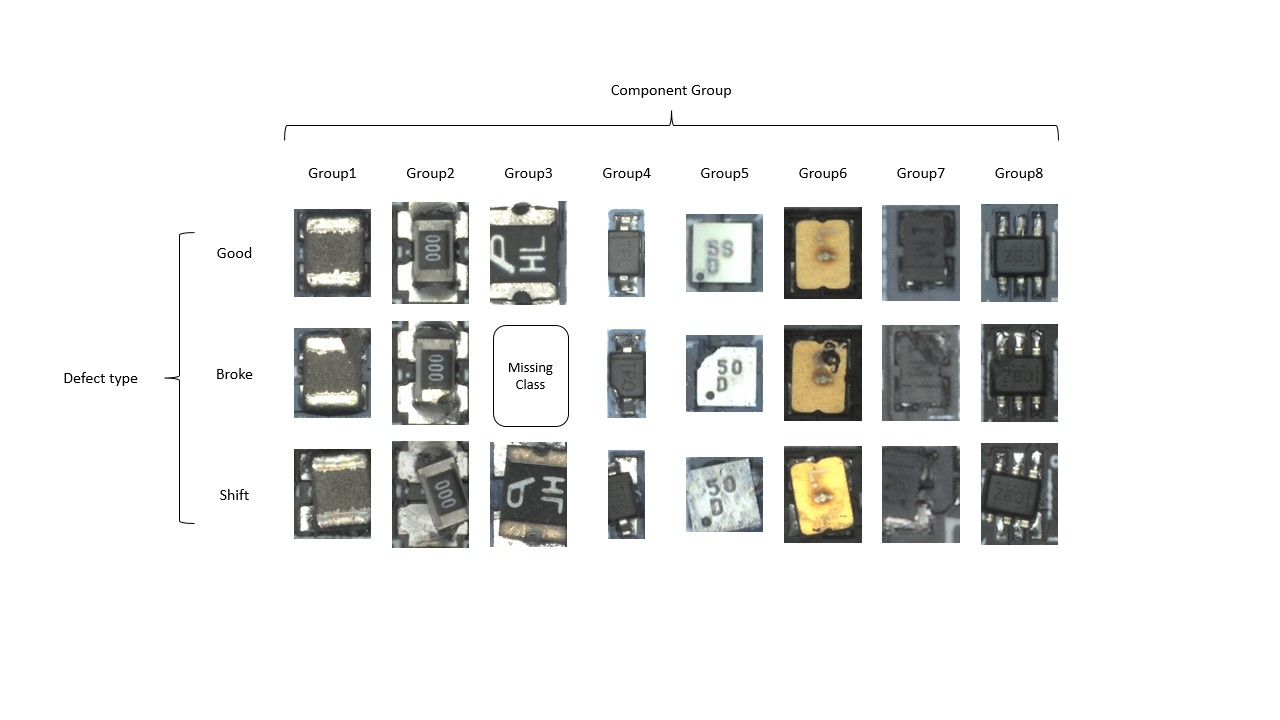
\includegraphics[width=1\linewidth]{Goal.jpg}
    \caption{The representation of component groups and defect types }
    \label{fig:enter-label}
\end{figure}

This study aims to employ an estimation method based on diffusion processes, utilizing a Compositional Class-to-image approach to generate defect images for new components (Broke Group3). The produced new components (Broke Group3) will be integrated into the defect component detection model to enhance the model's generalization ability to unseen images. Additionally, we implement Denoising Diffusion Implicit Models(DDIM)\cite{DDIM} sampling to expedite the generation process. The overarching goal is to provide direction and inspiration for future research in this domain.


\section{Contribution}
The contributions of this thesis are summarized in the following:
\begin{itemize}
    \item We propose a novel class-to-image generation method that reduces training time by eliminating the need for additional text pre-training models, such as CLIP\cite{CLIP}.
    \item Unlike traditional prompts requiring lengthy descriptions, our method does not rely on complex textual inputs yet is capable of producing accurate and exceptional images even in unseen contexts. This approach simplifies the generation process while ensuring both accuracy and diversity in the generated images.
    \item \textbf{Novelty in New Component Defect Generation Model}: Our study pioneers the use of the Compositional Conditional Diffusion method for generating defects in previously unseen new components. This groundbreaking approach represents a new contribution to the field, introducing a unique and innovative model for defect generation.
    \item \textbf{Practical Application Scenarios}: The potential real-world impact of our model, especially in the industrial welding domain, underscores its practical utility. This application-oriented contribution enhances the relevance and applicability of our research in addressing challenges within the welding industry.
\end{itemize}


\chapter{Related Work}
\label{chapter:relatedwork}

\section{Diffusion Model on Image Synthesis}
In the field of image synthesis, diffusion models [\cite{ho2020denoising}, \cite{song2020score}, \cite{mirza2014conditional}, \cite{sohl2015deep}] have achieved state-of-the-art performance. They have broken the long-standing dominance of GAN \cite{goodfellow2020generative} in image synthesis domain. Diffusion model have demonstrated outstanding performance in various domain of image synthesis, from the unconditional diffusion models \cite{ho2020denoising} to conditional diffusion models \cite{dhariwal2021diffusion}. Diffusion models have a wide range of applications, such as Image Super-Resolution [\cite{li2022srdiff}, \cite{saharia2022image}, \cite{rombach2022high}], Inpainting [\cite{rombach2022high}, \cite{saharia2022palette}], Image translation [\cite{ozbey2023unsupervised}, \cite{saharia2022palette}] and Editing [\cite{meng2021sdedit}]. These methods all implement the diffusion model, employing different conditional inputs and modifications to the architecture based on the conditional input. This allows the diffusion model to generate corresponding images based on different conditions. Text-to-Image generation is currently one of the most frequently discussed applications of diffusion models. Diffusion models need to generate corresponding image from a descriptive text. \cite{rombach2022high} utilized a pretrained text encoder CLIP \cite{radford2021learning} and used cross-attention to combine text information with diffusion model, generating real and diverse image based on text description. On the other hand, DALLE-2 \cite{ramesh2022hierarchical} proposed a two-state approach, involving a prior model capable of generating a CLIP-based image embedding based on a text caption, and a diffusion-based decoder that can generate an image conditioned on the produced image embedding. Imagen \cite{saharia2022photorealistic} employed a different text encoder T5 \cite{raffel2020exploring} which is a text-to-text transformer, they explored that a large language model trained on only text data is still very effective on text-to-image generation. In order to train with high-resolution images, \cite{rombach2022high} shifted the diffusion process to latent space to reduce computation resources. They first employed a pretrained autoencoder to encode images into latent space, then the diffusion process and the sampling process are conducting in the latent spaces. This method effectively reduces computational resources and can be applied to various tasks.


\section{Classifier-free guidance}
The original diffusion models were unconditional, meaning they couldn't be controlled by text or categories to generate images.\cite{dhariwal2021diffusion} proposed the classifier guidance method. During the training of the diffusion model, an additional classifier is trained on noisy samples. When sampling images, the diffusion model can be guided and generate images according to the class by leveraging the gradients from the classifier. This allows the diffusion model to generate images based on the specified class. This method need to train an additional classifier, the sampling quality is highly correlated with the classifier. \cite{ho2022classifier} proposed the proposed classifier-free guidance, allowing the diffusion model to generate images according to categories without the need for an additional classifier. By combining unconditional input and conditional input with a guidance scale $\omega$, the diffusion model can generate images based on categories without relying on an additional classifier.


\section{Compositional Zero-shot Learning (CZSL)}
Traditional Zero-Shot Learning (ZSL) [\cite{wang2019survey}, \cite{pourpanah2022review}, \cite{xian2018zero}, \cite{rahman2018unified}, \cite{xian2018feature}, \cite{han2021contrastive}] investigates classification tasks when there are no training samples available, but the semantics of new classes are known. One branch of research within ZSL is Compositional Zero-Shot Learning (CZSL) [\cite{xu2021zero}, \cite{yang2022decomposable}, \cite{lu2023decomposed}, \cite{saini2022disentangling}]. Given a known object concept, people can combine combine this object with various attribute to create different compositions. CZSL represents all attributes and objects as concept are available during training phase, the model needs to recognize the unseen compositions based on seen concepts and correctly classify them during validation or testing. \cite{chen2014inferring} trained a linear classifier of seen compositions and inferred unseen compositions form observed classifier using Bayesian framework. \cite{misra2017red} propose a simple approach which decomposed a complex concepts into multiple primitives and trained a binary linear classifier on each of these primitive. This method demonstrates our ability to infer a complex concept composed of two or more primitives, which motivate us on image selection framework. \cite{nagarajan2018attributes} propose a model based on the  concept of 'attributes as operators,' representing attribute-object composition. This model conditions transformations on attributes, incorporating it into an embedding learning model for identifying unseen compositions. \cite{yang2022decomposable} create a model that learn three spaces for the object, attribute and composition classifications.



\chapter{Preliminary}
\label{chapter:preliminary}
In this chapter, we will explain the process and mathematical principles of the denoising diffusion probabilistic model (diffusion model for short) \cite{ho2020denoising}, providing a basic understanding of diffusion models for better understanding the rest of this thesis.
\section{Diffusion model}
\label{sec:ddpm}
Diffusion model is a class of generative models that simulate a stochastic diffusion process where a simple initial distribution is transformed into a more complex distribution that represents the data distribution. They define a Markov chain of diffusion steps to slowly add random noise to data and then learn to reverse the diffusion process to construct desired data samples from the noise. Given a data point sampled from a real data distribution $x_0 \sim q(x)$, we add small amount of Gaussian noise $\epsilon$ to the original sample in $T$ steps, where $T$ is the total diffusion steps, $T \in \{1, 2, ..., T\}$, this produce a sequence of noisy sample $x_1, x_2, ..., x_T$ with different noise level and they all share the same dimension as $x_0$. The posterior $q(x_1, ...,  x_t | x_0)$, also known as the \textbf{forward diffusion process}, which converts the original data distribution $q(x_0)$ into a tractable prior distribution $q(x_t)$, typically Gaussian distribution. This process is set as a Markov chain, we can factorize the posterior as follows:
\begin{equation} \label{eq:1}
    q(x_1, ..., x_t | x_0) = \prod_{t = 1}^{T} q(x_t | x_{t-1}), \quad q(x_t | x_{t-1}) = \mathcal{N}(x_t; \sqrt{1 - \beta_t}x_{t-1}, \beta_t\textbf{I}),
\end{equation}
where $\beta_t \in (0, 1)$ is the variance schedule controlling the step size and can be regarded as a constant hyperparameter. Let $\alpha_t = 1 - \beta_t$ and $\overline{\alpha}_t = \prod_{i=1}^{t}\alpha_i$, then $x_t$ at arbitrary timestep $t$ can be expressed in a closed form:
\begin{equation} \label{eq:2}
    q(x_t|x_0) = \mathcal{N}(x_t;\sqrt{\overline{\alpha}_t}x_0, (1 - \overline{\alpha}_t)\textbf{I}),
\end{equation}
Equation \ref{eq:2} can be further reparameterized as
\begin{equation} \label{eq:3}
    x_t = \sqrt{\overline{\alpha}_t}x_0 + \sqrt{1 - \overline{\alpha}_t}\epsilon, \epsilon \sim \mathcal{N}(0, \textbf{I}),
\end{equation}

The \textbf{reverse diffusion process} gradually remove noise from noisy sample $x_t$, producing a slightly denoised sample $x_{t-1}$, since we cannot estimate $q(x_{t-1} | x_t)$, we need to learn a model $p_\theta$ to approximate $q(x_{t-1} | x_t)$.
\begin{equation} \label{eq:4}
    p_\theta(x_{t-1} | x_t) = \mathcal{N}(x_{t-1}; \mu_\theta(x_t, t), \Sigma_\theta(x_t, t))
\end{equation}
Here, $\theta$ denotes the model parameters and the mean $\mu_\theta(x_t, t)$ and the variance are modeled using deep neural networks. With this "denoising model", we can generate a data sample $x_0$ from a noise sample $x_t ~ q(x_t)$ sampled from prior distribution. 

When training the denoising model, \cite{ho2020denoising} try to maximize the variation lower bound (ELBO) on negative log-likelihood and utilize the Kullback-Leibler (KL) divergence.
\begin{equation} \label{eq:5}
\begin{split}
    \mathbb{E}_q[-\mathrm{log}p_\theta(x_0] \leq L \coloneqq \underbrace{\matchbb{E}_q[D_{KL}(q(x_T|x_0) || p_\theta(x_T))}_{L_T} + \\ \sum_{t=2}^{T}\underbrace{D_{KL}(q(x_{t-1}|x_t, x_0) || p_\theta(x_{t-1}|x_t))}_{L_{t-1}} - \underbrace{\mathrm{log}p_\theta(x_0|x_1)]}_{L_0}
\end{split}
\end{equation}

$L_T$ can be considered as a constant since $q$ does not have any parameters and $x_T$ is a Gaussian noise. $L_t$ can be considered as bringing two Gaussian distributions: $q(x_{t-1}|x_t, x_0) = \mathcal{N}(x_{t-1};\tilde{\mu}_t(x_t, x_0), \tilde{\beta}_tI)$ and $p_\theta(x_{t-1}|x_t) = \mathcal{N}(x_{t-1}; \mu_\theta(x_t, x_0), \Sigma_\theta)$ closer. Let:
\begin{equation} \label{eq:6}
    \tilde{\mu}_t(x_t, x_0) = \frac{\sqrt{\alpha}_t(1 - \overline{\alpha}_{t-1})}{1 - \overline{\alpha}_t}x_t + \frac{\sqrt{\overline{\alpha}_{t-1}}\beta_t}{1 - \overline{\alpha}_t}, \tilde{\beta}_t = \frac{1 - \overline{\alpha}_{t-1}}{1 - \overline{\alpha}_t}\beta_t \quad
\end{equation}
Based on the solving the KL divergence on the multivariate Gaussian distribution, $L_{t-1}$ can be rewritten as:

\begin{equation} \label{eq:7}
    L_{t-1} = \mathbb{E}_q[ \frac{1}{2\|\Sigma_\theta(x_t, t)\|_2^2} \|\tilde{\mu}_t(x_t, x_0) - \mu_\theta(x_t, t) \|^2 ] + C
\end{equation}

where $C$ is a constant, $\mu_\theta(x_t, x_0)$ is what we train to predict $\tilde{\mu}_t(x_t, x_0)$. 

\begin{equation} \label{eq:8}
    \mu_\theta(x_t, t) = \frac{1}{\sqrt{\alpha_t}}(x_t - \frac{1 - \alpha_t}{\sqrt{1 - \overline{\alpha}_t}}\epsilon_\theta(x_t, t))
\end{equation}

$\epsilon_\theta$ is the denoising model intended to predict $\epsilon_t$ from $x_t$. Since $x_t$ is available at training phase, we can try predict Gaussian noise term $\epsilon_t$ from the input $x_t$ as time step $t$ instead of predicting $\tilde{\mu}_t(x_t, x_0)$. The training objective of the denoising model becomes to predict the noise vector $\epsilon_t$ given noisy sample $x_t$ and timestep $t$. Bring Eq.(\ref{eq:6}), Eq.(\ref{eq:8}) into Eq.(\ref{eq:7}), Eq.(\ref{eq:7}) can be simplified to:

\begin{equation} \label{eq:9}
    L_{t-1} = \mathbb{E}_{x_0, \epsilon}[\frac{\beta_t^2}{2\alpha_t(1 - \overline{\alpha}_t\|\Sigma_\theta\|_2^2}\|\epsilon - \epsilon_\theta(\sqrt{\overline{\alpha}_t}x_0 + \sqrt{1 - \overline{\alpha}_t}\epsilon, t)\|^2]
\end{equation}

Through experiment results, \cite{ho2020denoising} discovered that beneficial to sample quality to train on a simpler objective function that ignored the weighting term:
\begin{equation} \label{eq:10}
    L_{simple} = \mathbb{E}_{x_0, \epsilon}[\|\epsilon - \epsilon_\theta(\sqrt{\overline{\alpha}_t}x_0 + \sqrt{1 - \overline{\alpha}_t}\epsilon, t)\|^2]
\end{equation}


Note that \cite{ho2020denoising} does not explicitly consider the $\Sigma_\theta$ in both training and inference;instead, it is set to $\beta_t$ or $\tilde{\beta}_t$. They found that predict $\Sigma_\theta$ could lead to training instability.

\section{Denoising Diffusion Implicit Models}
In practical applications, achieving high-quality images requires a larger timestep $T$, which can result in a time-consuming process for reverse diffusion process. To accelerate the reverse diffusion process, \cite{song2020denoising} introduced an approach that sacrifices diversity in exchange for faster inference. They discovered that the objective loss function in DDPM only relies on the marginal distribution $q(x_t|x_0)$, rather than on the joint distribution $q(x_{1:T}|x_0)$. They choose to use an alternative non-Markovian forward process, indexed by a real vector $\sigma \in \mathbb{R^T}$ the forward process is defined as:
\begin{equation} \label{eq:11}
    q_\sigma(x_{1:T}|x_0) = q_\sigma(x_T|x_0)\prod_{t=2}^{T}q_\sigma(x_{t-1}|x_t, x_0)
\end{equation}

where $q_\sigma(x_T|x_0) = \mathcal{N}(\sqrt{\alpha_T}x_0, (1 - \alpha_T)\textbf{I})$ for all $t > 1$,
\begin{equation} \label{eq:12}
    q_\sigma(x_{t-1} | x_t, x_0) = \mathcal{N}(x_{t-1}; \sqrt{\alpha_{t-1}}x_0 + \sqrt{1 - \alpha_{t-1} - \sigma_t^2} \frac{x_t - \sqrt{\alpha_t}x_0}{\sqrt{1 - \alpha_t}}, \sigma_t^2I)
\end{equation}
The forward process can be derived from Bayes' rule:
\begin{equation} \label{eq:13}
        q_\sigma(x_t | x_{t-1}, x_0) = \frac{q_\sigma(x_{t-1} | x_t, x_0)q_\sigma(x_t | x_0)}{q_\sigma(x_{t-1}|x_0)}
\end{equation}
In the reverse diffusion process, we can use following equation to generate $x_{t-1}$ from $x_t$
\begin{equation} \label{eq:14}
    x_{t-1} = \sqrt{\alpha_{t-1}}(\underbrace{\frac{x_t - \sqrt{1 - \alpha_t}\epsilon_\theta(x_t, t)}{\sqrt{\alpha_t}}}_{\text{predicted $x_0$}}) + \underbrace{\sqrt{1 - \alpha_{t-1} - \sigma_t^2} \cdot \epsilon_\theta(x_t, t)}_{\text{direction pointing to $x_t$}} + \underbrace{\sigma_t\epsilon_t}_{\text{random noise}}
\end{equation}

Let $\sigma_t^2 = \eta \cdot \tilde{\beta}_t$, we can consider $\eta$ as a hyperparameter to control the sampling stochasticity. When $\eta = 0$, the forward process becomes deterministic, the reverse process becomes a fixed procedure while the random noise term in Eq. \ref{eq:14} becomes zero.

Because DDIM has no specific forward process, we can use a forward process with a smaller number of steps to accelerate the model's generation process. We sample a subsequence $[\tau_1, \dots, \tau_S]$ with length $S$ from the original sequence $[1, \dots, T]$, then:
\begin{equation}
    q(x_{\tau_i}|x_0) = \mathcal{N}(\sqrt{\alpha_{\tau_i}}x_0, (1 - \alpha_{\tau_i})\textbf{I})
\end{equation}

The reverse process now generates samples according to $\tau$, because the length $S$ is much smaller than $T$, we can significantly accelerate the generation process.


In the following chapters, we will utilize the above equations to elucidate our approach.

\chapter{Proposed Method}
\label{chapter:method}


\section{Compositional Class label-to-Image Diffusion model (CCDM)}
\label{sec:CCDM}
Our model is a diffusion model conditioned on a compositional class label $c$, where $c = [c_1, \dots, c_n]$ is composed of a combination of labels from different categories. We use $n = 2$ and $n = 3$(two conditions and three conditions) for our model. In this chapter, we further decomposed our model into several components to introduce our approach: the denoising model , the conditioning module, and the compositional class encoder. As mentioned in Section \ref{sec:ddpm}, the denoising model is used to predict noise based on a compositional class label $c$, a timestep $t$ and a noisy sample $x_t$, with this model, we can use Eq. \ref{eq:14} to restore $x_t$ to $x_0$. The conditioning module is how we add conditional information into our denoising model, we employ four different architectures to integrate the information of compositional class labels.
The compositional class encoder is used to encode the compositional class label $c$, mapping the class label to a higher-dimensional space.
\begin{figure} [H]
    \centering
    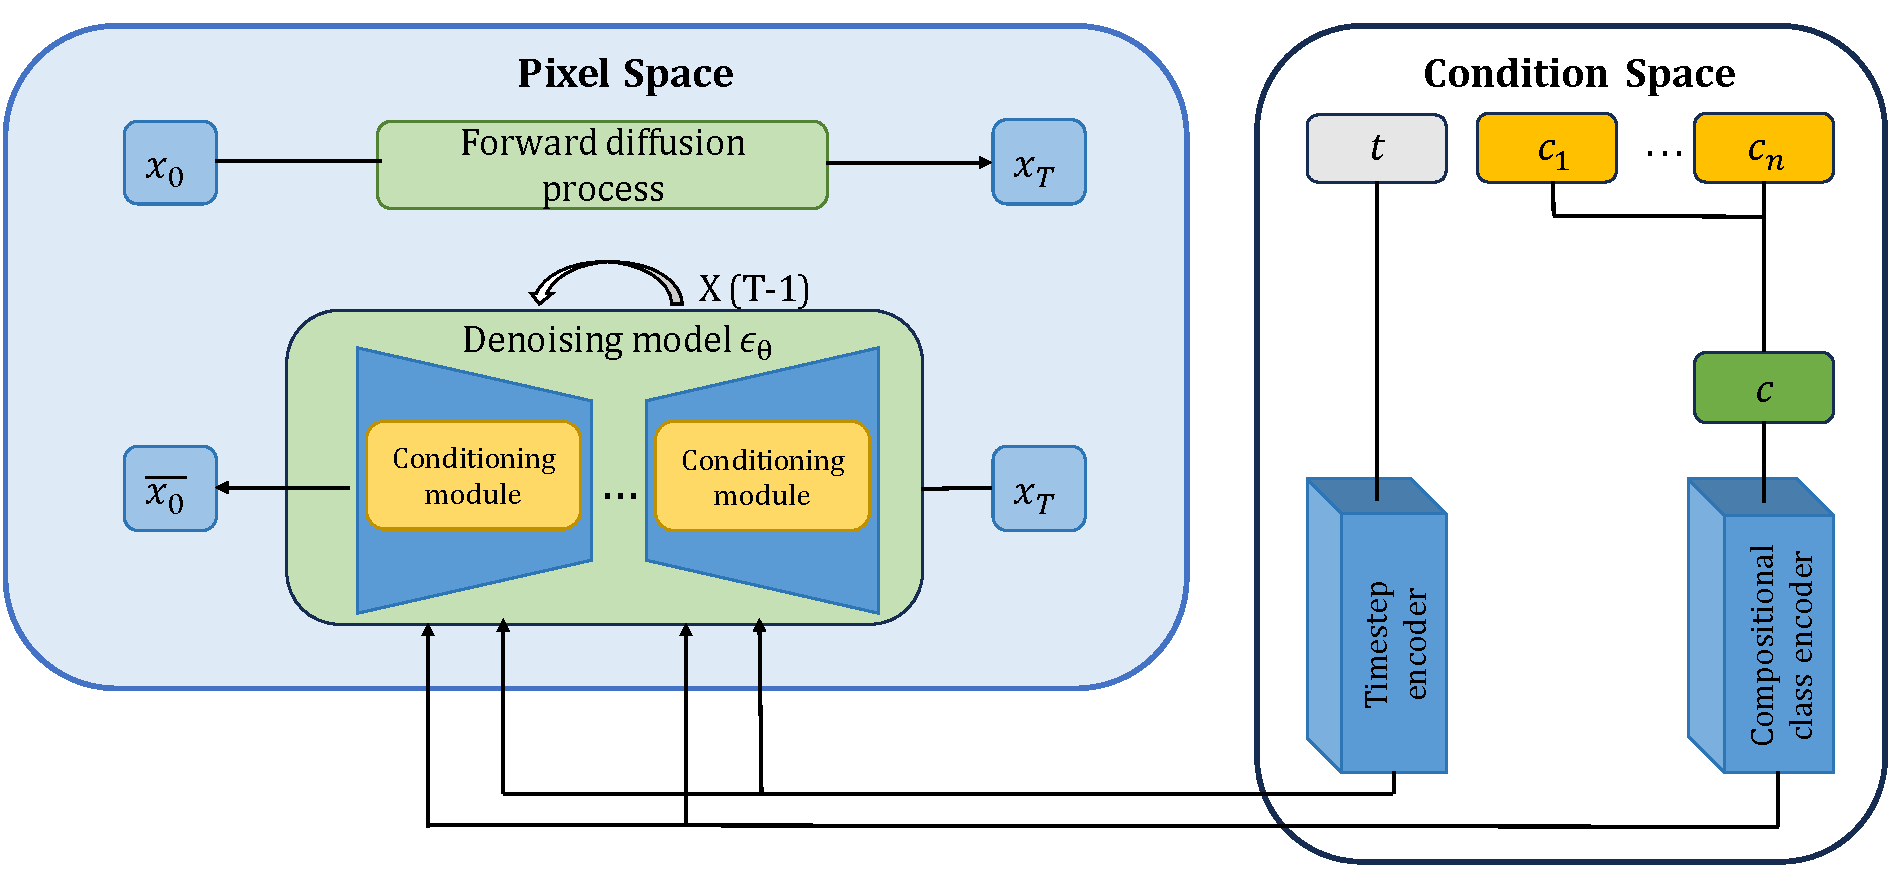
\includegraphics[width=0.8\linewidth]{figures/CCDMBlock.pdf}
    \caption{Block diagram of CCDM}
    \label{fig:CCDM}
\end{figure}
Figure \ref{fig:CCDM} illustrates the architecture of our model, the compositional class label will be encoded by the class encoder and integrate with the conditioned denoising model through the conditioner, and the conditioned denoising model will predict the noise term based on conditional information.

\section{Compositional class encoder}
In order to guide the diffusion model with compositional class information, we first use one-hot encoding to encode the compositional class label for different categories. Given $c = (c_1, c_2, c_3, ...)$ is the compositional class label, the compositional class encoder is illustrated as the follows:
\begin{figure} [H]
    \centering
    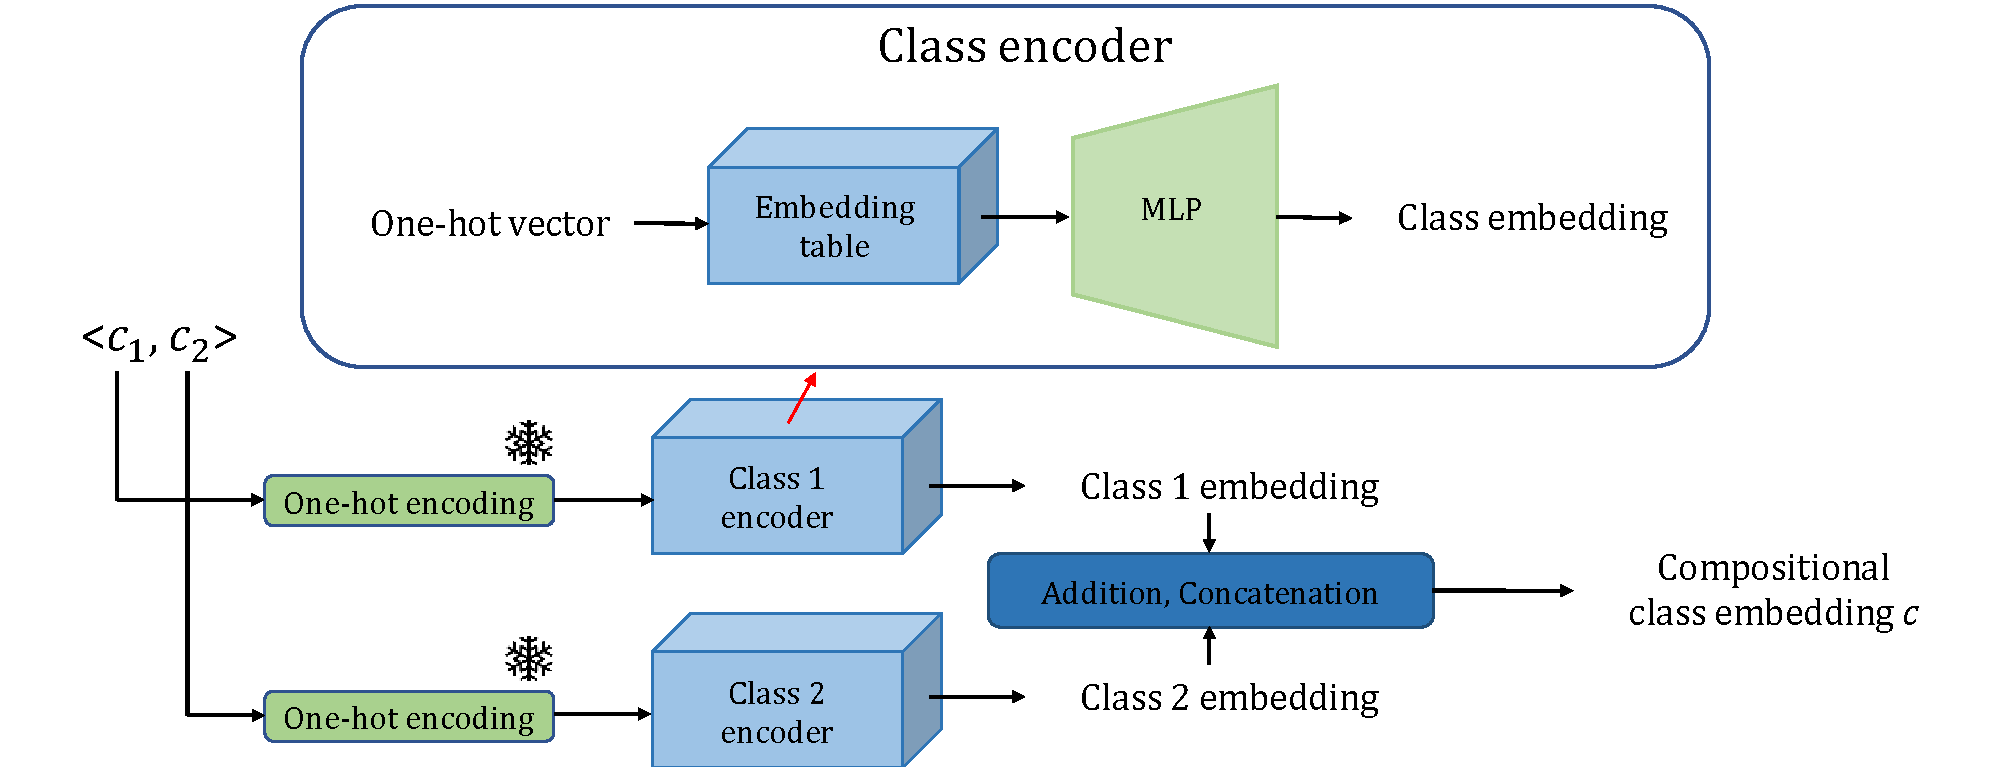
\includegraphics[width=1\linewidth]{figures/Class encoder.pdf}
    \caption{Compositional class encoder}
    \label{fig:class encoder}
\end{figure}

For each category's class label, we first encode them using one-hot encoding. Then, we use an embedding table and MLP to encode the one-hot vector. Finally, we sum or concatenate these class embeddings based on different conditioning modules. Figure \ref{fig:class encoder} illustrates how we encode compositional class labels using two category class labels.

\section{Denoising model}
According to Chapter \ref{chapter:preliminary}, we added a compositional class label $c$ to guide our denoising model. We modify Eq.\ref{eq:10} to cooperate with compositional class label $c$ and sampled image according to the compositional label $c$. The modified loss function will be:
\begin{equation}
    L_{simple} = \mathbb{E}_{x_0, \epsilon}[\|\epsilon - \epsilon_\theta(\sqrt{\overline{\alpha}_t}x_0 + \sqrt{1 - \overline{\alpha}_t}\epsilon, t, c)\|^2]
\end{equation}
Our denoising model $\epsilon_\theta$ now has three inputs, which are the noisy sample $x_t$, timestep $t$ and the compositional label $c$ instead of only $x_t$ and $t$. The training and sampling procedure are illustrated as the follows:
\begin{algorithm}
\caption{Training CCDM}
\label{training}
\vspace{2mm}
\begin{algorithmic}[1]
\Repeat: \vspace{2mm}
    \State $(x_0, c) \sim p(x, c)$  \vspace{2mm}
    \State $c \leftarrow \varnothing \text{ with probability } p_{uncond}$
    \State $t \sim Uniform(\{1, \dots, T\})$ \vspace{2mm}
    \State $\epsilon \sim \mathcal{N}(0, \textbf{I})$ \vspace{2mm}
    \State $x_t = \sqrt{\overline{\alpha}_t}x_0 + \sqrt{1 - \overline{\alpha}_t}\epsilon$ \vspace{2mm}
    \State Take a gradient step on $ \nabla_{\theta} \| \epsilon - \epsilon_\theta(\sqrt{\overline{\alpha}_t}x_0 + \sqrt{1 - \overline{\alpha}_t}\epsilon, t, c) \|^2 $ \vspace{2mm}
    \Until converged \vspace{2mm}
\end{algorithmic}
\end{algorithm}

\begin{algorithm}
\caption{Sampling}
\label{sampling}
\vspace{2mm}
\begin{algorithmic}[1]
\Require $\omega:$ guidance scale \vspace{2mm}
\Require $c:$ Compositional class label for compositional generation
\Require $\eta:$ hyperparameter controlling sampling stochasticity \vspace{2mm}
\State $x_t \sim \mathcal{N}(0, \textbf{I})$ \vspace{2mm}
\For{t = $S, \dots, 1$} \vspace{2mm}
    \State $\epsilon \sim \mathcal{N}(0, \textbf{I})$ if $t > 1$, else $\epsilon = 0$ \vspace{2mm}
    \State $\sigma_t = \eta \cdot \tilde{\beta}_t$ \vspace{2mm}
    \State $\tilde{\epsilon}_t = (1 + \omega)\underbrace{\epsilon_\theta(x_t, t, c)}_{\text{conditional noise}} - \omega\underbrace{\epsilon_\theta(x_t, t, \varnothing)}_{\text{unconditional noise}}$ \vspace{4mm}
    \State $x_{t-1} = \sqrt{\alpha_{t-1}}(\frac{x_t - \sqrt{1 - \alpha_t}\tilde{\epsilon}_t}{\sqrt{\alpha_t}}) + \sqrt{1 - \alpha_{t-1} - \sigma_t^2} \cdot \tilde{\epsilon}_t + \sigma_t\epsilon_t$ \vspace{2mm}
\EndFor \vspace{2mm}
\State \textbf{return} $\overline{x_0}$ \vspace{2mm}
\end{algorithmic} 
\end{algorithm}

\begin{figure} [H]
    \centering
    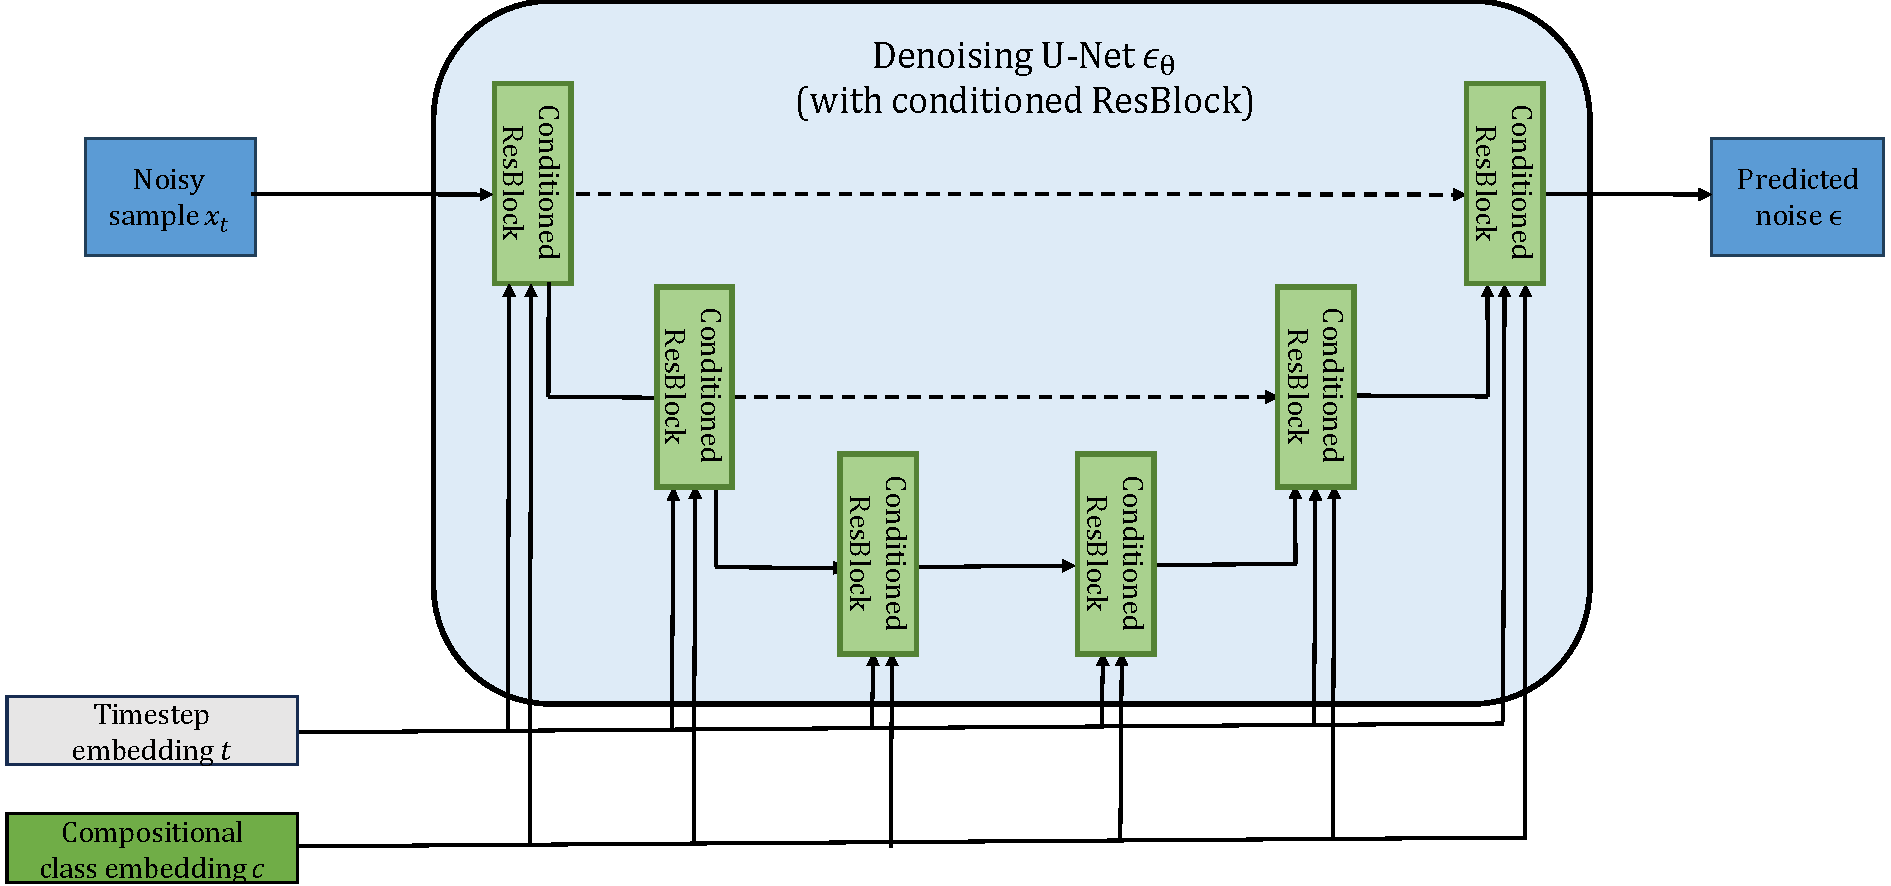
\includegraphics[width=1\linewidth]{figures/UNetRes.pdf}
    \caption{Conditioned denoising U-Net with conditioned ResBlock}
    \label{fig:unetres}
\end{figure}

\begin{figure} [H]
    \centering
    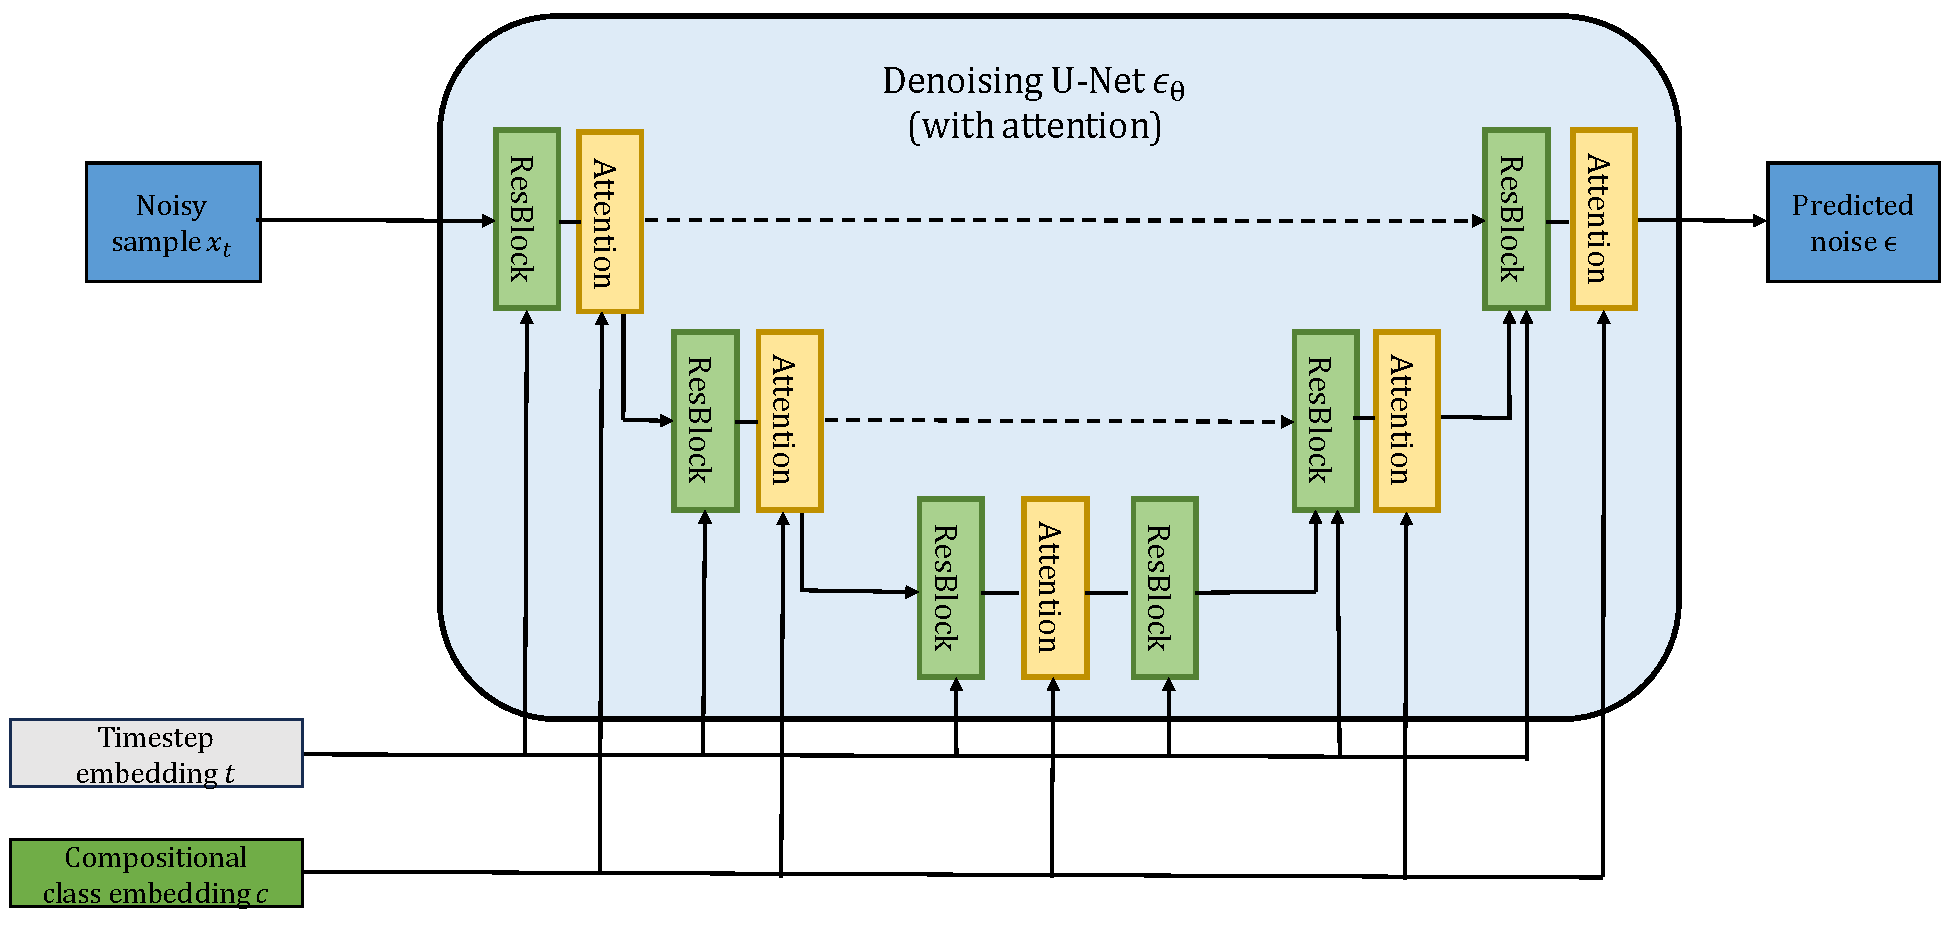
\includegraphics[width=1\linewidth]{figures/UNetAttention.pdf}
    \caption{Conditioned denoising U-Net with attention}
    \label{fig:unetattention}
\end{figure}


Figure \ref{fig:unetres} and figure \ref{fig:unetattention} shows how to integrate conditional information with each residual block in the conditioned denoising U-Net. The difference between these two U-Net architectures lies in the location where condition information is incorporated.

\section{Conditioning module}
\label{subsec: conditioning module}
There are various methods to incorporate conditional information into the denoising model. Drawing inspiration from numerous papers, we implemented four different conditioning modules in our model. In the following schematic diagram, we will illustrate how we use the information from compositional class labels to guide our model. Before introducing these conditioning modules, we need to establish definitions for some symbols. Let $h$ be the hidden state, $t$ be the timestep embedding vector, $c$ be the compositional class embedding vector and $proj$ be the linear projection layer.
\subsection{Addition (Add)}
Follow DDPM\cite{ho2020denoising} implementation, we preform element-wise addition on projected timestep embedding and compositional class embeddings into each residual block. We define the conditioning module as Add$(h, t, c)$, then
\begin{equation}
    \text{Add}(h, t, c) = h + proj(t) + proj(c)
\end{equation}

\begin{figure} [H]
    \centering
    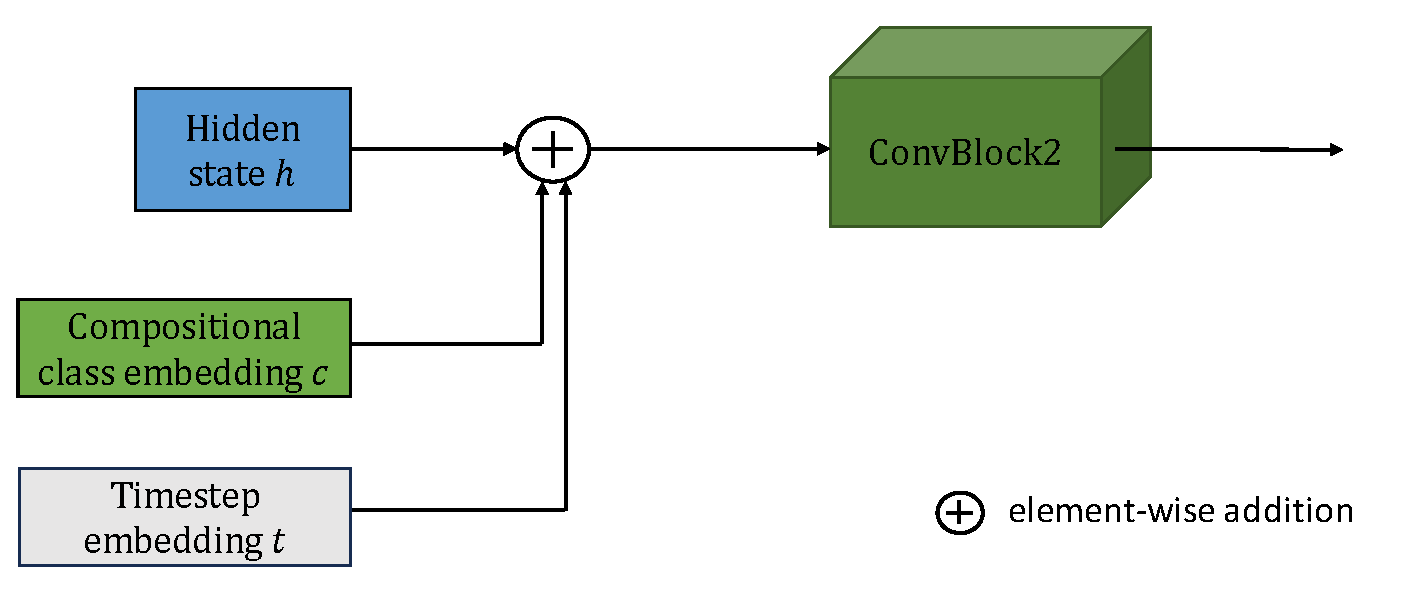
\includegraphics[width=0.8\linewidth]{figures/Add.pdf}
    \caption{Addition}
    \label{fig:add}
\end{figure}
Figure \ref{fig:add} shows how we integrate hidden state $h$ and conditional information. In each residual block, we add projected timestep embedding and projected compositional class embedding into $h$, where $h$ is the output of the first convolution block. We call this conditioning module \textbf{Add} for the rest of this thesis.
\subsection{Adaptive Group Normalization (AdaGN)}
Follow \cite{nichol2021improved} implementation, we also implement this module on our model, let $y^{\prime} = proj(y + t)$ and $y^{\prime} = [y_s, y_b]$, which we split $y^{\prime}$ into two vectors with the same dimension, then the conditioning module is illustrated as the follows:
\begin{equation}
    \text{AdaGN}(h, t, c) = (1 + c_s)\text{GroupNorm}(h) + c_b
\end{equation}
\begin{figure} [H]
    \centering
    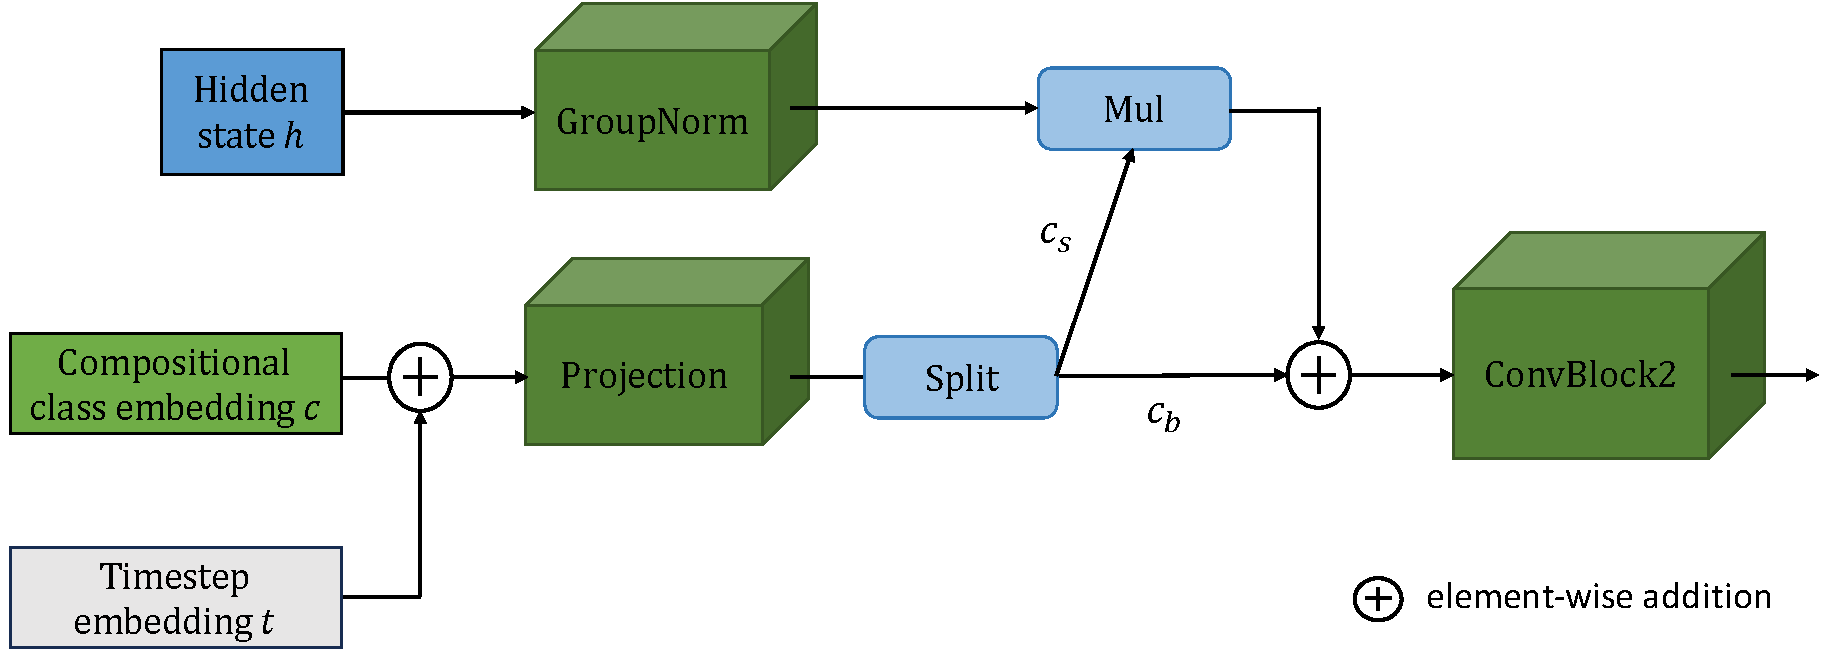
\includegraphics[width=0.8\linewidth]{figures/AdaGN.pdf}
    \caption{Adaptive Group Normalization}
    \label{fig:adagn}
\end{figure}
Figure \ref{fig:adagn} illustrates the procedure of adaptive group normalization, the projection layer maps the original dimension, which is 512, to 512 * 2, while the split operation divides the vector, originally of dimension 1024, into two 512-dimensional vectors.

\subsection{Image Class concatenation (IC)}
We concatenate compositional class embedding $y$ with hidden state $h$ to add conditional information guidance, then we use a bottleneck layer to reduce dimension after concatenation, details are illustrated as the follows:
\begin{figure} [H]
    \centering
    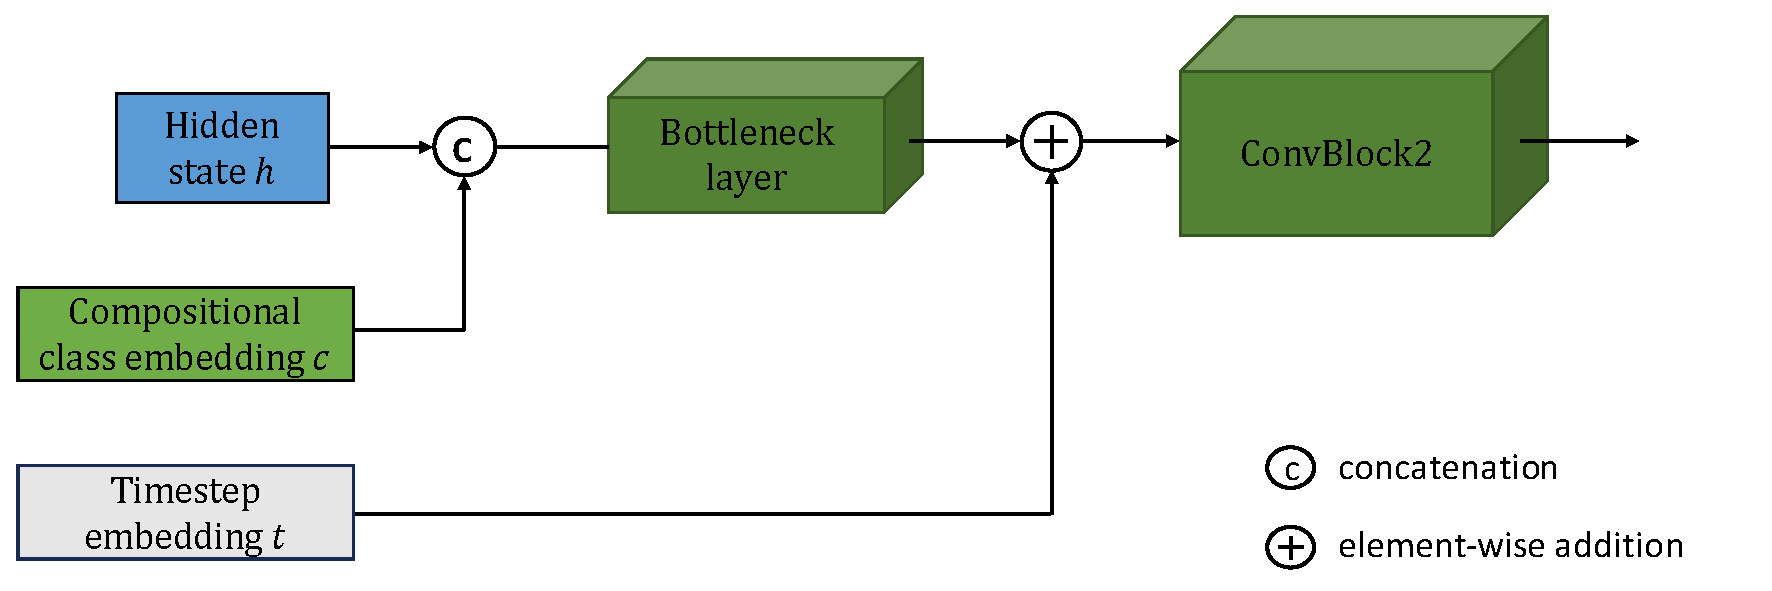
\includegraphics[width=0.8\linewidth]{figures/IC.pdf}
    \caption{Image class concatenation}
    \label{fig:ic}
\end{figure}
Follow \cite{rombach2022high} implementation of super-resolution and inpainting diffusion model. We concatenate concatenate compositional class embedding $c$ with hidden state $h$ in diffusion process.Figure \ref{fig:ic} illustrates how we integrate timestep embedding $t$ and compositional class embedding $y$ with hidden state $h$. We first combine the hidden state and compositional class information using concatenation. Then, we use a bottleneck layer for dimensionality reduction, restoring it to the original dimension. Finally, we incorporate the timestep information through element-wise addition. 

\subsection{Cross Attention (CA)}
Follow \cite{rombach2022high} implementation, we use an shallow spatial transformer composed by $N$ transformer blocks, each block consists of a multi-head self-attention layer, a position-wise feedforward network and a multi-head cross-attention layer.
\begin{figure} [H]
    \centering
    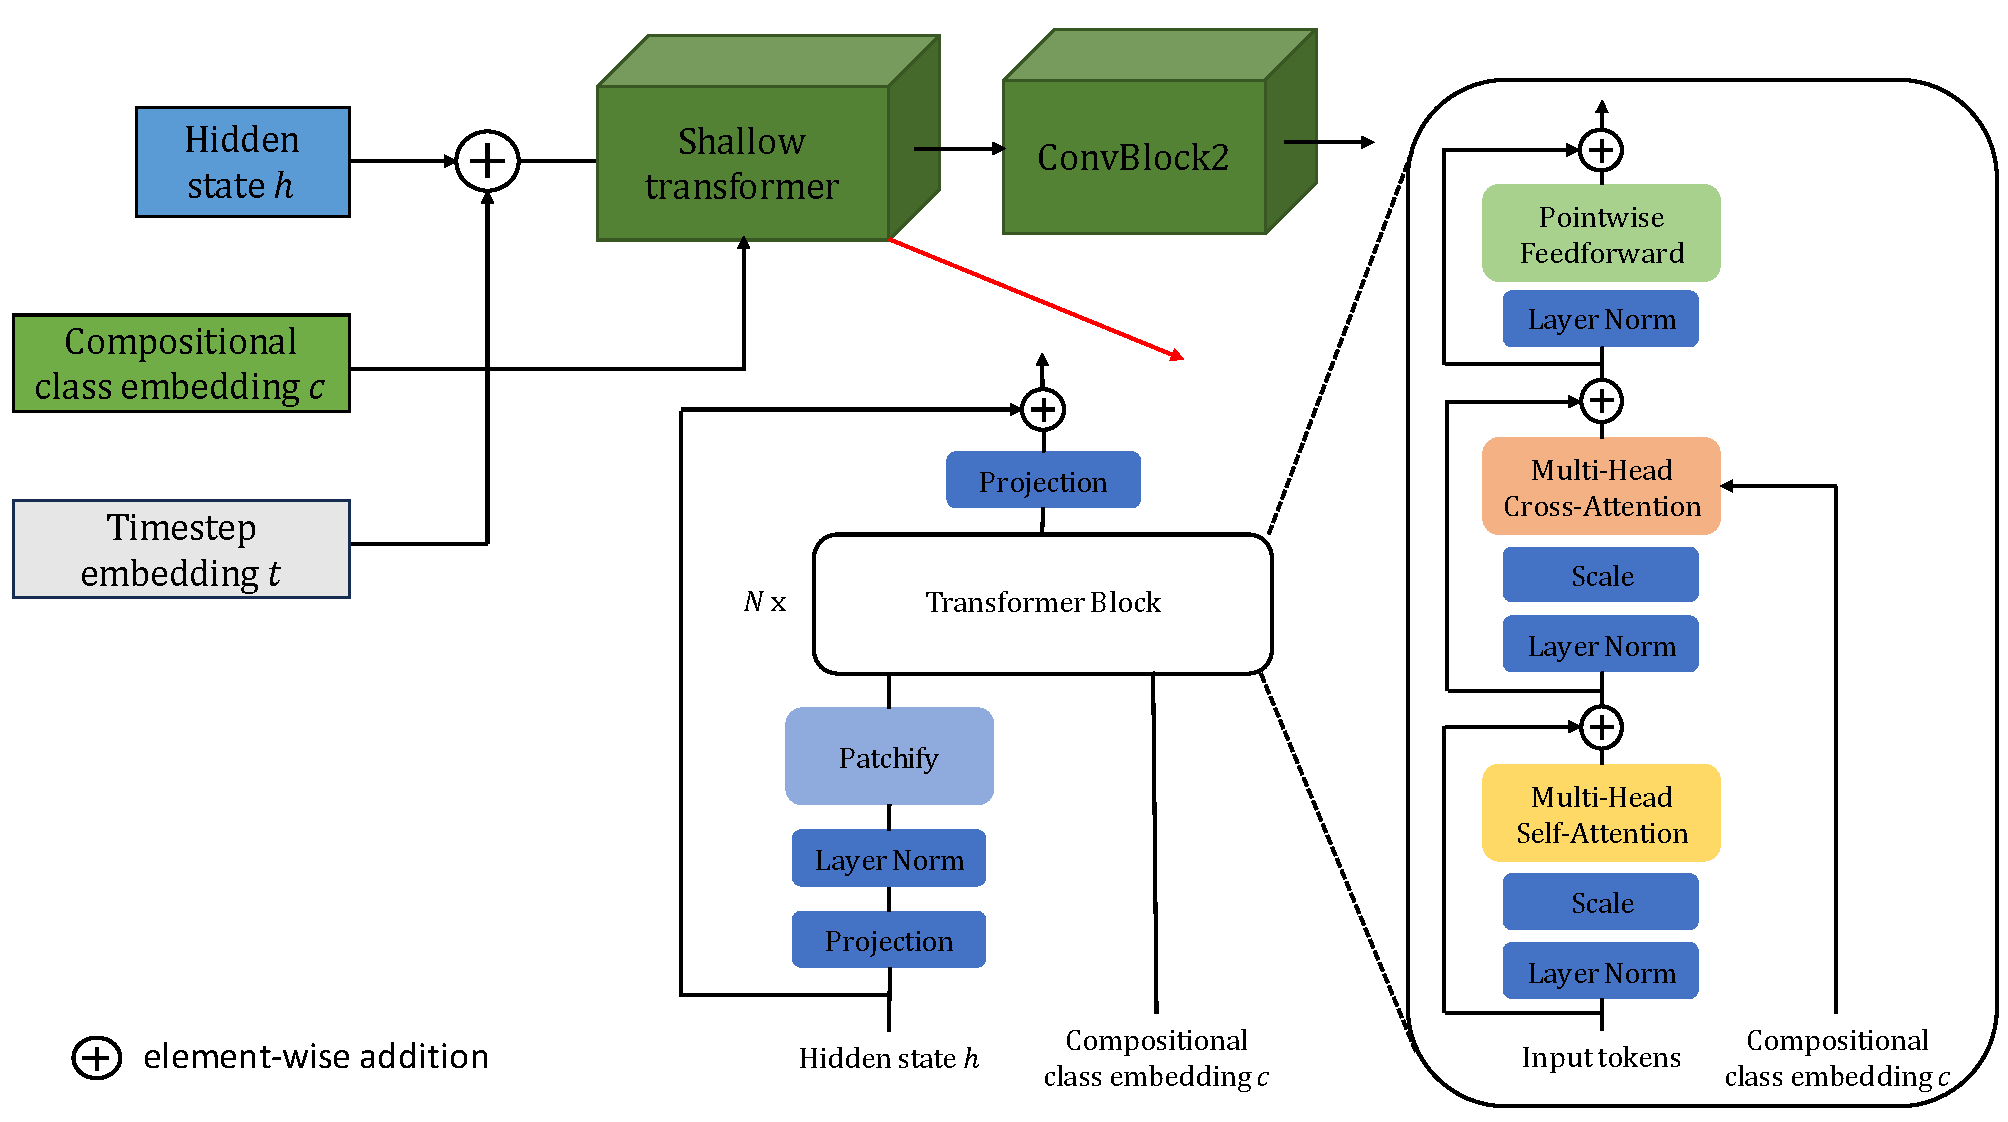
\includegraphics[width=0.8\linewidth]{figures/CA.pdf}
    \caption{Cross attention}
    \label{fig:ca}
\end{figure}
Figure \ref{fig:ca} illustrates the architecture of spatial transformer and transformer block, note that the compositional class embedding $y \in \mathbb{R}^{B \times 1 \times D_{emb}}$ is extended from the original compositional class embedding $y \in \mathbb{R}^{B \times D_{emb}}$ by adding a new dimension.

\section{Image Selector}
\label{sec:selector}
Although CCDM has the capability of compositional zero-shot image generation, not every generated image aligns perfectly with the unseen compositional class label. Sometimes, the images produced by the model may exhibit deviations. Therefore, we require a framework to assess the performance of the model.

 We introduced an image selection framework to assess the model. Following \cite{misra2017red}, we separately trained binary classifiers for the object and attribute of unseen compositions. Using ``Heel Slipper`` as an example, we would train a ``Heel`` binary classifier and a ``Slipper`` binary classifier. These classifiers are then utilized to filter the images generated by CCDM.
To ensure the reliability of these classifiers, we first generated N unseen composition images using CCDM. Subsequently, we utilized these classifiers to select images that match the unseen compositions. We then manually verified whether the selected images indeed matched the criteria.
\begin{figure} [H]
    \centering
    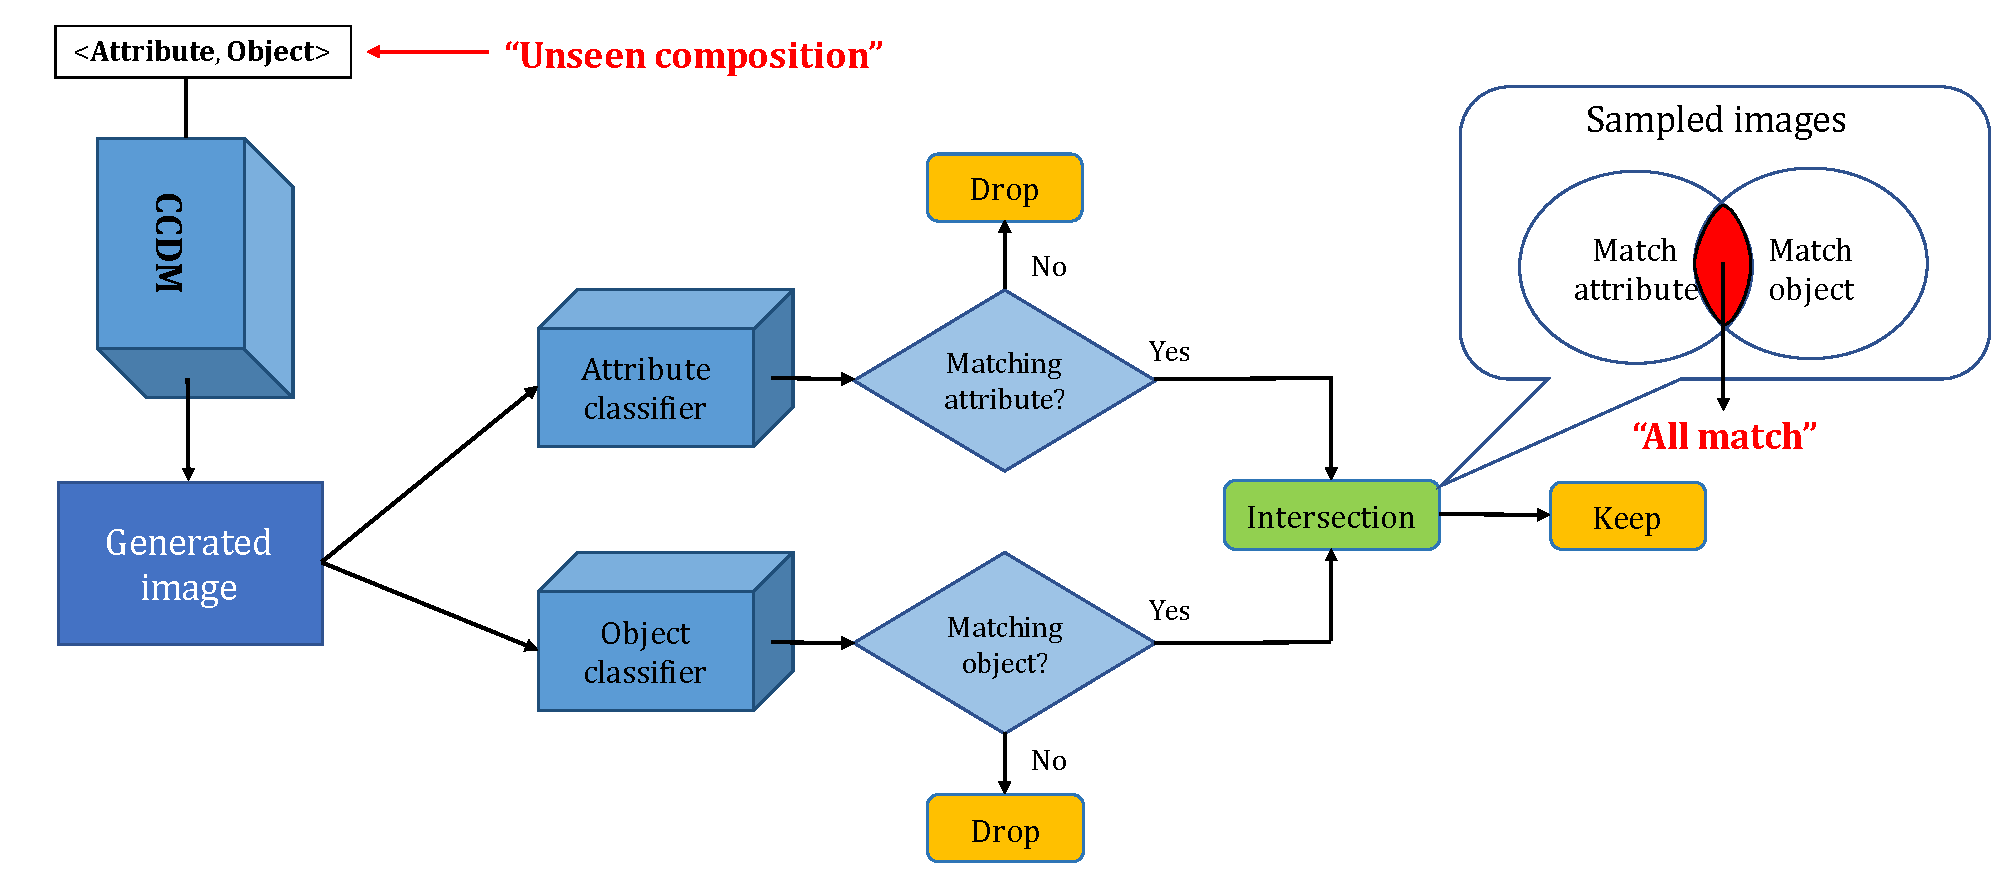
\includegraphics[width=1\linewidth]{figures/Image selector.pdf}
    \caption{Image selector on unseen composition}
    \label{fig:selection}
\end{figure}

Figure \ref{fig:selection} illustrates how we evaluate a generated image. After generating images using CCDM based on unseen compositional class labels, each generated image undergoes evaluation by multiple binary classifiers to determine whether it matches the description of the class label. 


\chapter{Experiment Results}
\label{chapter:experiments}

\section{Dataset preparation}
\label{sec:dataset}
For conducting experiments on Compositional zero-shot image generation, we utilized several datasets, including publicly available datasets and ones we generated ourselves. In the initial stages to validate the feasibility of our ideas, we started with a very simple dataset that we generated ourselves. After achieving success on this dataset, we proceeded to use publicly available datasets. In the following sections, we will provide detailed introductions for each dataset.


\subsection{Shape Color Dataset}
\label{subsec:shapecolor}
This dataset is generated by the python OpenCV library, includes various geometric shapes of different colors.
\begin{itemize}
    \item \textbf{Two condition setting:} We use geometric shapes as the object category. There are a total of 6 object classes: Circle, Oval, Triangle, Rectangle, Pentagon, and Hexagon. We use color as the attribute category, with a total of 6 attribute classes: Red, Green, Blue, Yellow, Purple, and Black, resulting in a total of 36 compositions, As illustrated in table \ref{tab:twocondshape}. Each of them has 1000 training samples. Each training sample is a 64 * 64 pixel image, the size and the location of the geometric object are randomized.
    
    \begin{table} [H]
        \centering
        \begin{tabular}{c|c|c}
             & Condition 1 (Color) & Condition 2 (Geometric shape)\\
             \hline
             Labels & Circle, Hexagon, Oval, Pentagon, Rectangle, Triangle & Black, Blue, Green, Purple, Red, Yellow \\
        \end{tabular}
        \caption{Two condition setting of Shape Color dataset}
        \label{tab:twocondshape}
    \end{table}
    
    \item \textbf{Three condition setting:} Continuing with the two-condition setting, we use the size of the objects as a new category, with a total of 3 classes: Big, Medium, Small. This results in a total of 108 compositions, As illustrated in table \ref{tab:threecondzappo}. Each of them has 1000 training samples. Each training sample is a 64 * 64 pixel image.

    \begin{table} [H]
    \resizebox{\columnwidth}{!}{\begin{tabular} {c|c|c|c}
        \centering
             & Condition 1 (Size) & Condition 2 (Color) &  Condition 3 (Geometric shape)\\
             \hline
            Labels & Big, Medium, Small & Circle, Hexagon, Oval, Pentagon, Rectangle, Triangle & Black, Blue, Green, Purple, Red, Yellow \\
        \end{tabular}}
        \caption{Three condition setting of Shape Color dataset}
        \label{tab:threecondshape}
    \end{table}
\end{itemize}

\subsection{UT-Zappos50K}
The UT-Zappos50K dataset comprises a total of 50,025 images of footwear, categorized into four main types: Shoes, Boots, Slippers, and Sandals. These images are further divided based on their functional types. We have restructured the dataset and removed some ambiguous data in the dataset for our experiments, leaving us with 47,917 images for training.
\begin{itemize}
    \item \textbf{Two condition setting:} We retain the original four major categories as object category, introducing a new attribute category based on the presence or absence of heels, dividing it into two attribute classes: Heel and Flat. This results in a total of 8 compositions. As illustrated in table \ref{tab:twocondzappo}. 
    \begin{table} [H]
        \centering
        \begin{tabular}{c|c|c}
             & Condition 1 (Shoe height) & Condition 2 (Shoe type) \\
             \hline
             Labels & Heel, Flat & Boot, Shoe, Sandal, Slipper \\
        \end{tabular}
        \caption{Two condition setting of UT-Zappo50K dataset}
        \label{tab:twocondzappo}
    \end{table}
    \item \textbf{Three condition setting:} The images in the dataset were initially captured from a consistent perspective, so we horizontally flipped half of the data to introduce different shooting angles as a new category, with a total of 2 classes: Left, Right. Continuing with the two-condition setting, resulting a total of 16 compositions. As illustrated in table \ref{tab:threecondzappo}.
    \begin{table} [H]
        \centering
        \begin{tabular}{c|c|c|c}
             & Condition 1 (Filming angle) & Condition 2 (Shoe height) & Condition 3 (Shoe type)\\
             \hline
            Labels & Left, Right & Heel, Flat & Boot, Shoe, Sandal, Slipper \\
        \end{tabular}
        \caption{Three condition setting of UT-Zappo50K dataset}
        \label{tab:threecondzappo}
    \end{table}
\end{itemize}

\subsection{CelebFaces Attributes Dataset}
\label{subsec:celeba}
CelebFaces Attributes Dataset(CelebA) is a large-scale face attributes dataset with 202599 face images, each with 40 binray attribute annotations. 
\begin{itemize}
    \item \textbf{Two condition setting:}We use two of these attributes as our object category: Male and Female. For the attribute category, we use 4 of these attributes: Black Hair, Brown Hair, Blond Hair, Gray Hair. This results in a total of 8 compositions. As illustrated in table \ref{tab:twocondceleba}.
    \begin{table} [H]
        \centering
        \begin{tabular}{c|c|c}
             & Condition 1 (Hair color) & Condition 2 (Gender) \\
             \hline
             Labels & Black hair, Gray hair, Blond hair, Brown hair &  Male, Female \\
        \end{tabular}
        \caption{Two condition setting of CelebA dataset}
        \label{tab:twocondceleba}
    \end{table}
    \item \textbf{Three condition setting:}Continuing with the two-condition setting, we use hair style as a new category, dividing it into 2 classes: Wavy Hair and Straight Hair. This results in a total of 16 compositions. As illustrated in table \ref{tab:threecondceleba}
    
    \begin{table} [H]
        \centering
        \begin{tabular}{c|c|c|c}
             & Condition 1 (Hair style) & Condition 2 (Hair color) & Condition 3 (Gender)\\
             \hline
            Labels & Straight hair, Wavy hair & Black hair, Gray hair, Blond hair, Brown hair &  Male, Female \\
        \end{tabular}
        \caption{Three condition setting of CelebA dataset}
        \label{tab:threecondceleba}
    \end{table}
\end{itemize}



\section{Experiment setup}
\subsection{Training Diffusion model}
To train our model, we refer to the common hyperparameter settings of the stable diffusion model to configure the hyperparameters of our model. We used the following default hyperparameters: the training epoch was set to 100, the initial learning rate was set to $6 \times 10^{-5}$ with 10 warm-up epochs and the cosine learning rate scheduler was used for more stable training. For the optimization, we used AdamW optimizer with weight dacay values $10^{-4}$.

Diffusion process related hyperparameters are descride as follows. For the forward diffusion process, we set $T = 50$ for experiments with 2D Point Dataset, for the rest of experiments, we set $T = 1000$.For all experiments, the variance $\beta_T$ was set to $10^{-4}$ increasing linearly to 0.02. For the reverse process, we used classifier-free DDIM to sample images, the guildance strength $\omega$ to 1.8, $\eta$ was set to 0 and the samples were generated in 100 steps.

As for the hyperparameters related to the denoising models and the conditioner, they are described as the follows: For the denoising model used in 2D Point Dataset related experiments, we implemented the denoising model as a MultiLayer Perceptron (MLP) with three fully connected layers. For rest of the experiments, we implemented U-Net as our denoising model, we set the number of residual blocks to 2 in each downsample or upsample block. We set the base channel to 128 and the channel multiplier to [1, 2, 2, 2]. For the conditioner of cross attention , we used the same architecture in stable diffusion, which is a unmasked transformer, the number of attention head was set to 4 and the attention resolutions were set to [32, 16, 8].

The training images were all resized to 64 x 64 with RGB channels. All experiments were conducted on two NVIDIA Tesla V100 GPU.
The hyperparameter configuration for each architecture are illustrated with the following table.


\begin{table} [H]
    \centering
    \begin{tabular}{cc} 
         \hline
         & CCDM (with Conditioned ResBlock) \\
         \hline
         Diffusion steps & 1000\\
         Noise Schedule & linear \\
         Base Channels & 128 \\
         Number of Residual Blocks & 2\\
         Channel Multiplier & 1,2,2,2 \\
         Batch Size & 64 \\
         Epochs & 100 \\
         Learning Rate & $6 \times 10^{-5}$ \\
         Embedded Dimension & 512 \\
    \bottomrule[0.5mm]
    \end{tabular}
    \caption{Hyperparameters for CCDM(without attention) trained on the Shape Color Dataset, UT-Zappo50K, CelebA.}
    \label{tab:ccdmcondresblock}
\end{table}

\begin{table} [H]
    \centering
    \begin{tabular}{cc} 
         \hline
         & CCDM (with attention) \\
         \hline
         Diffusion steps & 1000\\
         Noise Schedule & linear \\
         Base Channels & 128 \\
         Number of Residual Blocks & 2\\
         Channel Multiplier & 1,2,2,2 \\
         Batch Size & 64 \\
         Epochs & 100 \\
         Learning Rate & $6 \times 10^{-5}$ \\
         Embedded Dimension & 512 \\
         \hline
         Number of Attention Heads & 4 \\
         CA-resolutions & 32, 16, 8 \\
         Transformer Depth & 1 \\
    \bottomrule[0.5mm]
    \end{tabular}
    \caption{Hyperparameters for CCDM(with attention) trained on the Shape Color Dataset, UT-Zappo50K, CelebA.}
    \label{tab:ccdmattention}
\end{table}

\subsection{Sampling}
During the generation phase, we utilize DDIM \cite{ho2020denoising} to accelerate the generation process. For each dataset, there is an unseen composition. We employ the trained CCDM to generate 1000 unseen compositional images using the unseen compositional class label. The hyperparameters used are illustrate in table \ref{tab:samplinghyperparameters}
\begin{table} [H]
    \centering
    \begin{tabular}{c|c}
        Hyperparameters & \\
        \hline
         Diffusion steps & 100\\
         Batch size & 200\\
         Guidance scale $\omega$ & 1.8\\
         Sampling stochasticity $\eta$ & 0\\
         Number of samples & 1000\\
    \end{tabular}
    \caption{Hyperparameters in sampling phase}
    \label{tab:samplinghyperparameters}
\end{table}

\subsection{Dataset splitting}
To train the binary classifiers within the image selector framework, we divided the available data into a training set and a validation set. We used 80 percent of the available data as the training set and 20 percent of the available data as the validation set. We used the training set to train the binary classifiers and tested them on the validation set.

\section{Evaluation Metrics}
Deep learning tasks require specific evaluation metrics that are tailored to the particular problem at hand. To evaluate the performance of CCDM, our focus is on the model's ability to generate unseen composition images. Therefore, we did not utilize the traditional Frechet Inception Distance(FID) \cite{heusel2017gans} for evaluation. During testing, the unseen composition images generated by CCDM are denoted as $N$, the unseen composition images selected by unseen image selector are denoted as $N_{select}$.
\begin{itemize}
    \item \textbf{Classification accuracy of binary classifier:} In order to assess whether the generated images by the model align with the description of unseen compositional class labels, we train a supervised binary classifier for each category class label of the unseen compositional class label. We evaluate the performance of each classifier based on its accuracy on the test dataset of each compositional class label.
    \item \textbf{Sample accuracy:} Follow \cite{liu2022compositional} evaluation metric, the images generated by CCDM are filtered by the image selector to choose those that match the unseen compositions. Sample accuracy is employed to assess CCDM's ability to generate unseen compositions, which includes whether the images generated by CCDM match the unseen compositional class label and the class label of each condition.
    \begin{equation}
        \text{Sample accuracy} = \frac{N_{select}}{N}
    \end{equation}
\end{itemize}


\section{Experiment results}
We designed various architectures for testing on each dataset, including both two-condition and three-condition settings. In this comparison, we evaluated different conditioning mechanisms and class encoder structures using sample accuracy. The detailed dataset settings are provided section \ref{sec:dataset} in  The detailed conditioning mechanisms are provided in figure \ref{fig:add}, figure \ref{fig:adagn}, figure \ref{fig:ic}, figure \ref{fig:ca}.

\subsection{Experiment results on shape color dataset}
After the successful experimentation with the 2D point dataset, we proceeded to test our model with more complex and higher-dimensional data, which is a major application of modern diffusion models:image generation. We began with our self-created shape color dataset \ref{subsec:shapecolor}, employing various architectures for the generation of unseen composition images. We designed different scenarios to assess the performance of CCDM

\begin{figure} [H]
    \centering
    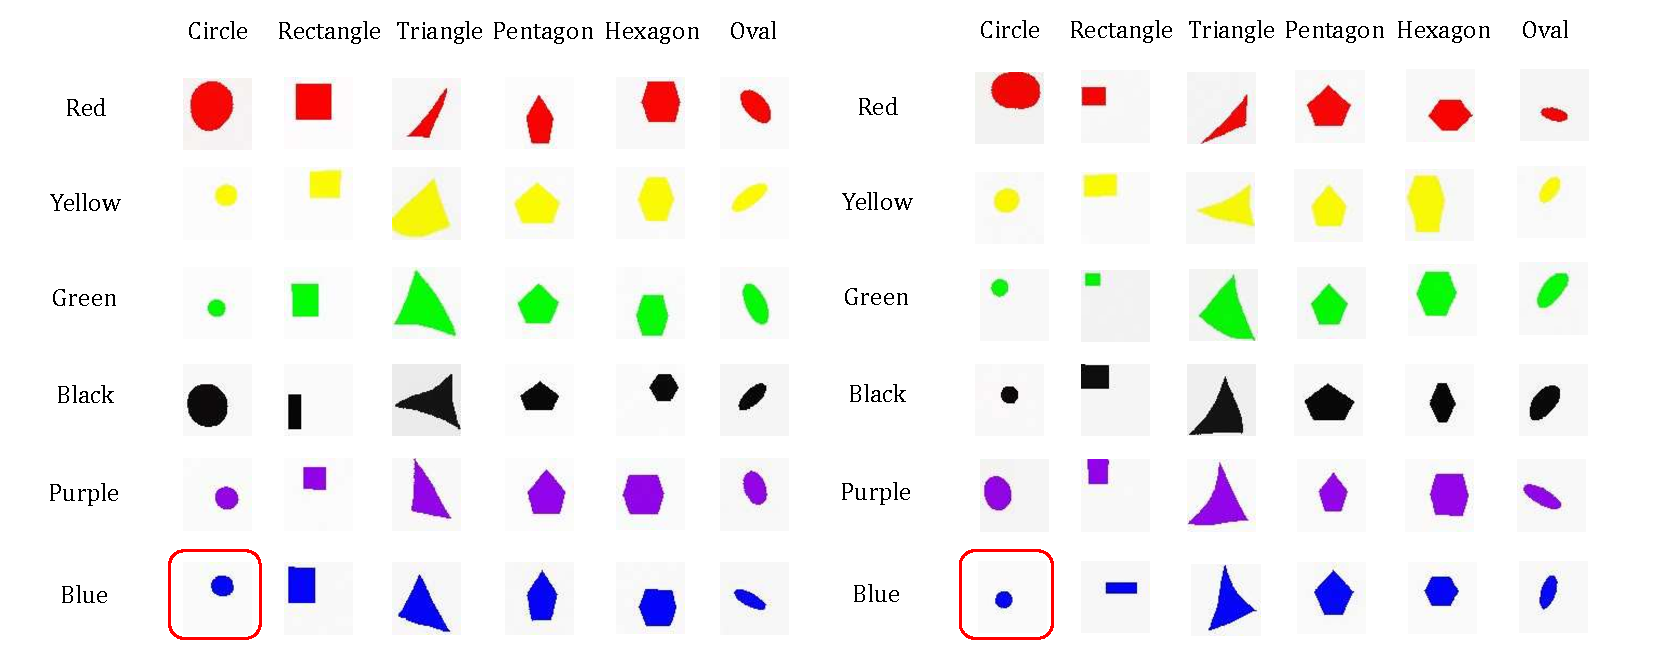
\includegraphics[width=1\linewidth]{figures/ShapeColor1.pdf}
    \caption{Under two condition setting of shape color dataset. Samples generated from CCDM, the unseen composition images are represented in red boxes.}
    \label{fig:sample_1}
\end{figure}

\begin{table} [H]
    \centering
    \begin{tabular}{cc}
         Classifier & Accuracy on validation set($\%$) $\uparrow$ \\
         \hline
         Blue classifier & 100 \\
         Circle classifier & 100 \\
         
    \end{tabular}
    \caption{Accuracy of binary classifiers within image selector(Two conditions setting)}
    \label{ShapeColorBinAcc}
\end{table}

\begin{table} [H]
    \centering
    \begin{tabular}{cccc}
         Architecture & $c_1$ accuracy $\uparrow$ & $c_2$ accuracy $\uparrow$ & All Corrects accuracy $\uparrow$ \\
         \hline
         Add & 0.54 & 0.55 & 0.31\\
         AdaGN & 0.46 & 0.76 & 0.35\\
         IC & 0.87 & \textbf{0.80} & \textbf{0.70}\\
         CA & \textbf{0.99} & 0.61 & 0.61\\
    \end{tabular}
    \caption{Architecture comparison on Shape Color Dataset (Two conditions setting)}
    \label{ShapeColorAcc}
\end{table}


\begin{figure} [H]
    \centering
    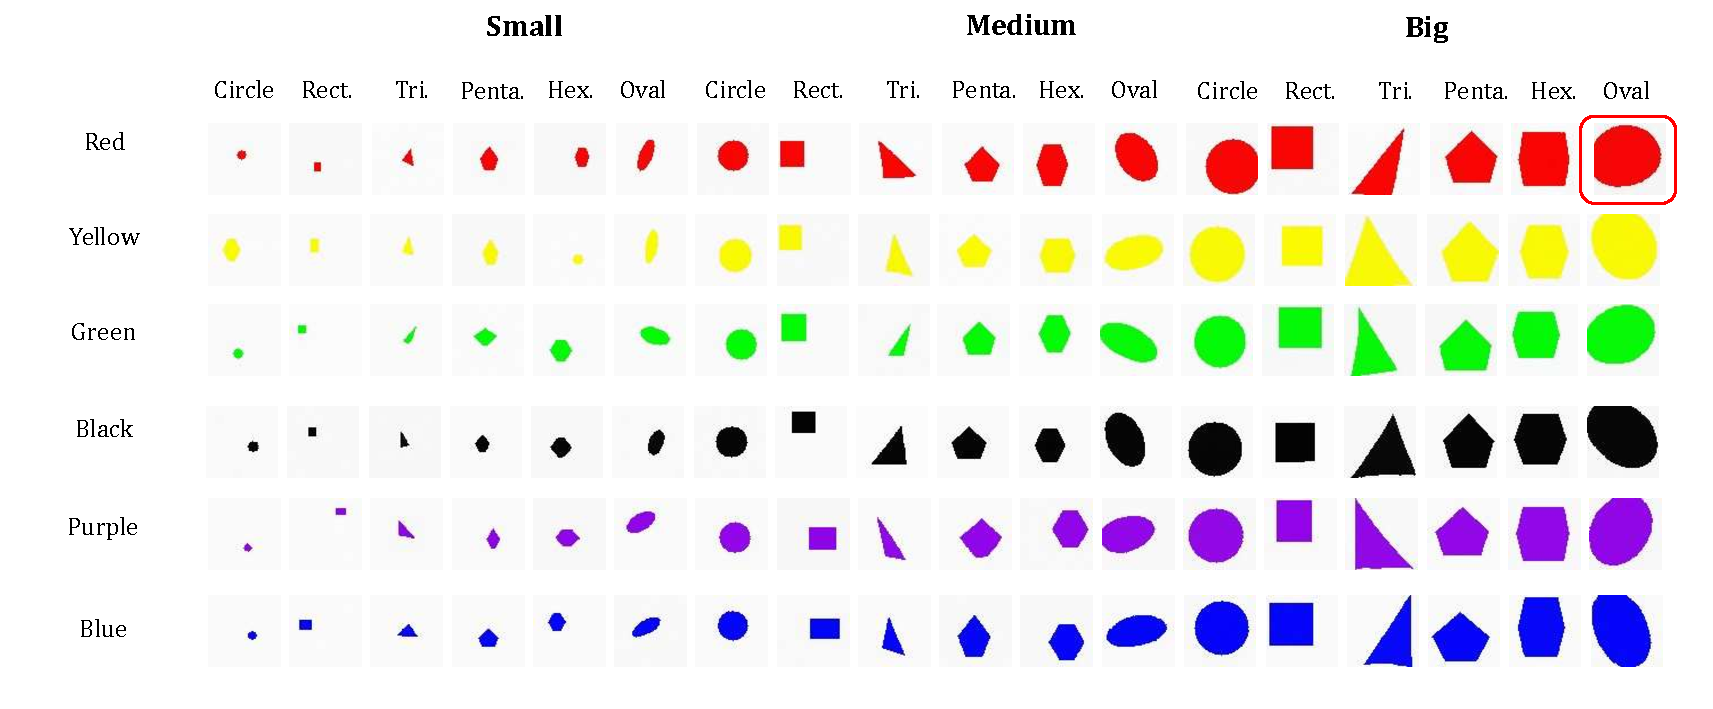
\includegraphics[width=1\linewidth]{figures/ShapeColor2.pdf}
    \caption{Samples of seen and unseen composition images generated from different architecture of CCDM, the unseen composition is represented by images enclosed in red boxes.}
    \label{fig:sample_3}
\end{figure}

From the experimental results in figure \ref{fig:sample_1} and figure \ref{fig:sample_3}, CCDM were able to successfully generate images of compositions that were not present during training. The results for seen compositions were also very promising across the board. These results also boosts our confidence in CCDM's ability to generalize to unseen compositions.

\begin{table} [H]
    \centering
    \begin{tabular}{cc}
         Classifier & Accuracy on validation set($\%$) $\uparrow$ \\
         \hline
         Big classifier & 100 \\
         Red classifier & 100 \\
         Oval classifier & 99.80 \\
    \end{tabular}
    \caption{Accuracy of binary classifiers within image selector(Three conditions setting)}
    \label{ShapeColorBinAccTri}
\end{table}

\begin{table} [H]
    \centering
    \begin{tabular}{ccccc}
         Architecture & $c_1$ accuracy $\uparrow$ & $c_2$ accuracy $\uparrow$ & $c_3$ accuracy $\uparrow$ & All Corrects accuracy $\uparrow$ \\
         \hline
         Add  & \textbf{1.0} & \textbf{1.0} & 0.98 & 0.98\\
         AdaGN & 0.99 & 0.99 & 0.96 & 0.95\\
         IC & \textbf{1.0} & \textbf{1.0} & \textbf{1.0} & \textbf{1.0}\\
         CA & \textbf{1.0} & 0.99 & \textbf{1.0} & 0.99\\
    \end{tabular}
    \caption{Architecture comparison on Shape Color Dataset (Three conditions setting)}
    \label{ShapeColorTriAcc}
\end{table}


\subsection{Experiment results on UT-Zappo50K}
After confirming that CCDM possesses the capability to generate unseen compositions, we proceeded to test CCDM on real-world datasets, specifically public datasets. We conducted tests on UT-Zappo50K, a common dataset in CZSL (Zero-Shot Learning), and made some modifications to the dataset structure. We examined CCDM's performance under different structures and scenarios. However, we encountered a challenge—instability in unseen composition generation. CCDM's ability to generate unseen composition images was not consistently stable under certain circumstances in these datasets. To address this, we employed an image selector to mitigate the issue. We will compare various architectures and evaluate their ability to generate unseen compositions. Detailed parameters of each architecture are provided in table \ref{tab:ccdmcondresblock}, table \ref{tab:ccdmattention}.

\begin{figure} [H]
    \centering
    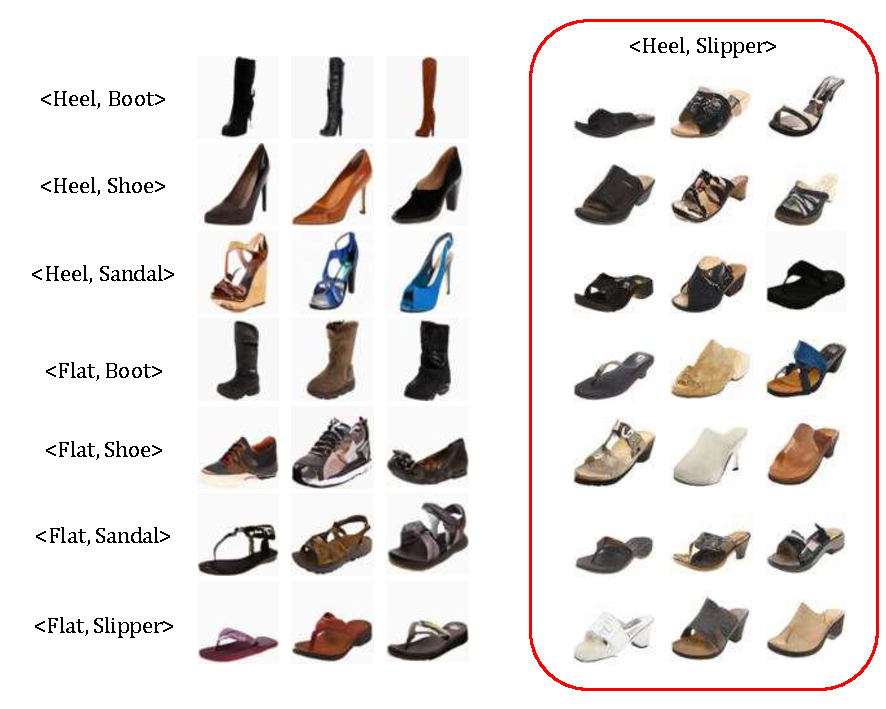
\includegraphics[width=1\linewidth]{figures/Zappo1.pdf}
    \caption{Under two condition setting of UT-Zappo50K. Samples generated from CCDM, the unseen composition images are represented in red boxes.}
    \label{fig:sample_6}
\end{figure}

\begin{table} [H]
    \centering
    \begin{tabular}{cc}
         Classifier & Accuracy on validation set($\%$) $\uparrow$ \\
         \hline
         Heel classifier & 87.50 \\
         Slipper classifier & 93.87 \\
         
    \end{tabular}
    \caption{Accuracy of binary classifiers within image selector(Two conditions setting)}
    \label{ZappoBinAcc}
\end{table}

\begin{table} [H]
    \centering
    \begin{tabular}{c|ccc}
         Architecture & $c_1$ accuracy $\uparrow$ & $c_2$ accuracy $\uparrow$ & All Corrects accuracy $\uparrow$ \\
         \hline
         Add & 0.17 & \textbf{0.9} & 0.07\\
         AdaGN & 0.28 & 0.71 & 0.06 \\
         IC & 0.31 & 0.86 & \textbf{0.18} \\
         CA & \textbf{0.62} & 0.50 & 0.16 \\
    \end{tabular}
    \caption{Architecture comparison on UT-Zappo50K Dataset (Two conditions setting)}
    \label{tab:Zappo50KAcc}
\end{table}


\begin{figure} [H]
    \centering
    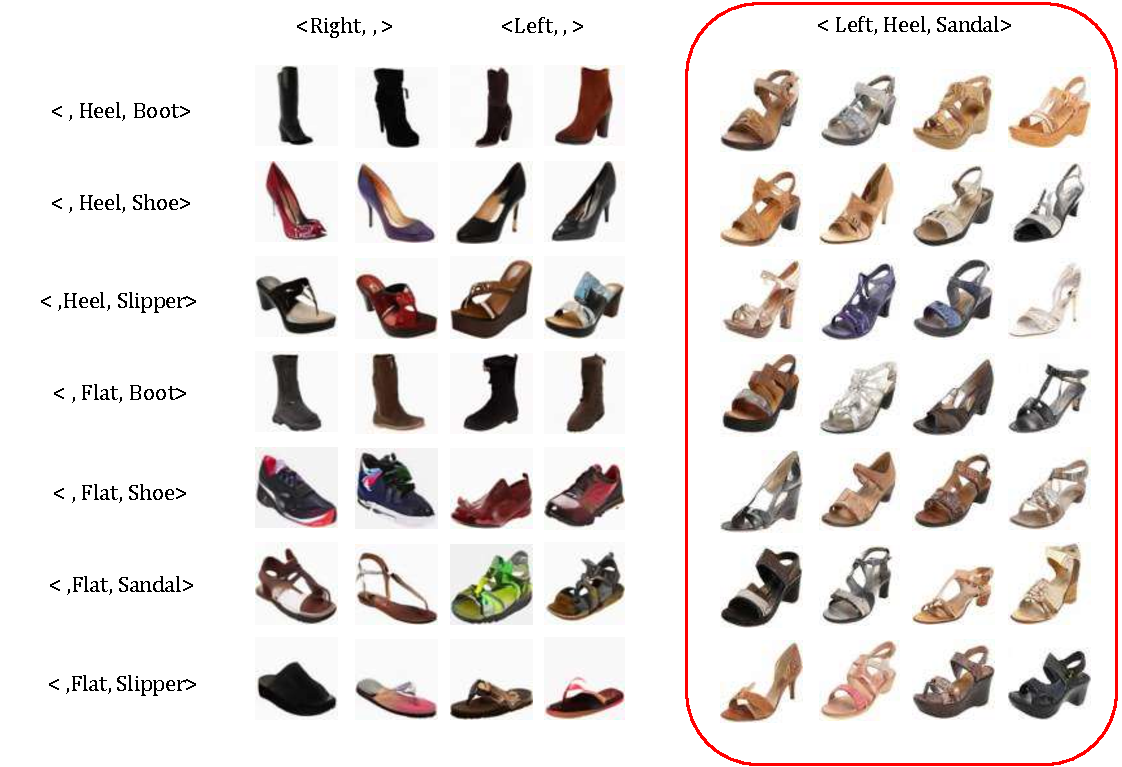
\includegraphics[width=1\linewidth]{figures/Zappo2.pdf}
    \caption{Under three condition setting of UT-Zappo50K. Samples generated from CCDM, the unseen composition images are represented in red boxes.}
    \label{fig:sample_8}
\end{figure}

\begin{table} [H]
    \centering
    \begin{tabular}{cc}
         Classifier & Accuracy on validation set($\%$) $\uparrow$ \\
         \hline
         Left classifier & 100 \\
         Heel classifier & 87.50 \\
         Sandal classifier & 95.60 \\
    \end{tabular}
    \caption{Accuracy of binary classifiers within image selector(Three conditions setting)}
    \label{ZappoBinAccTri}
\end{table}

\begin{table} [H]
    \centering
    \begin{tabular}{ccccc}
         Architecture & $c_1$ accuracy $\uparrow$ & $c_2$ accuracy $\uparrow$ & $c_3$ accuracy $\uparrow$ & All Corrects accuracy $\uparrow$ \\
         \hline
         Add  & \textbf{1.0} & 0.32 & 0.93 & 0.27\\
         AdaGN & \textbf{1.0} & 0.75 & 0.5 & \textbf{0.29}\\
         IC & \textbf{1.0} & 0.25 & \textbf{0.94} & 0.21\\
         CA & \textbf{1.0} & \textbf{0.99} & 0.06 & 0.06 \\
    \end{tabular}
    \caption{Architecture comparison on UT-Zappo50K Dataset (Three conditions setting)}
    \label{tab:Zappo50KTriAcc}
\end{table}

Figures \ref{fig:sample_6} and figure \ref{fig:sample_8} demonstrate CCDM's performance on the UT-Zappo50K dataset. It accurately generates unseen composition images, showcasing varied styles similar to real shoes. This illustrates CCDM's applicability to real-world datasets.In the results of table \ref{tab:Zappo50KAcc}, where $c_1$ represents "Heel," a subtle attribute, similar to the observations in table \ref{tab:CelebATriAcc}, we notice similar trends. In table \ref{tab:Zappo50KTriAcc}, where $c_2$ still represents "Heel" and $c_3$ represents "Sandal," we observe that Slipper and Sandal have many similarities in the UT-Zappo50K dataset. This leads to CCDM generating incorrect images, with many resembling slippers. Through experimentation, we confirm that CCDM possesses the capability of compositional zero-shot image generation. However, CCDM struggles with generating features that are subtle or have low separability, resulting in lower accuracy when generating such samples.


\subsection{Experiment results on CelebA}
To demonstrate that CCDM's ability to generate unseen compositions is not limited to a single case, we chose to conduct tests on the CelebA dataset, a well-known dataset in the field of image synthesis. CelebA Dataset is renowned for its comprehensive annotations, which facilitated a smoother experimental process. We selected several attributes from the original CelebA dataset to serve as different conditions, as detailed in \ref{subsec:celeba}. We conducted various tests on CCDM using different architectures and scenarios on the CelebA dataset.Detailed parameters of each architecture are provided in table \ref{tab:ccdmcondresblock}, table \ref{tab:ccdmattention}.

\begin{figure} [H]
    \centering
    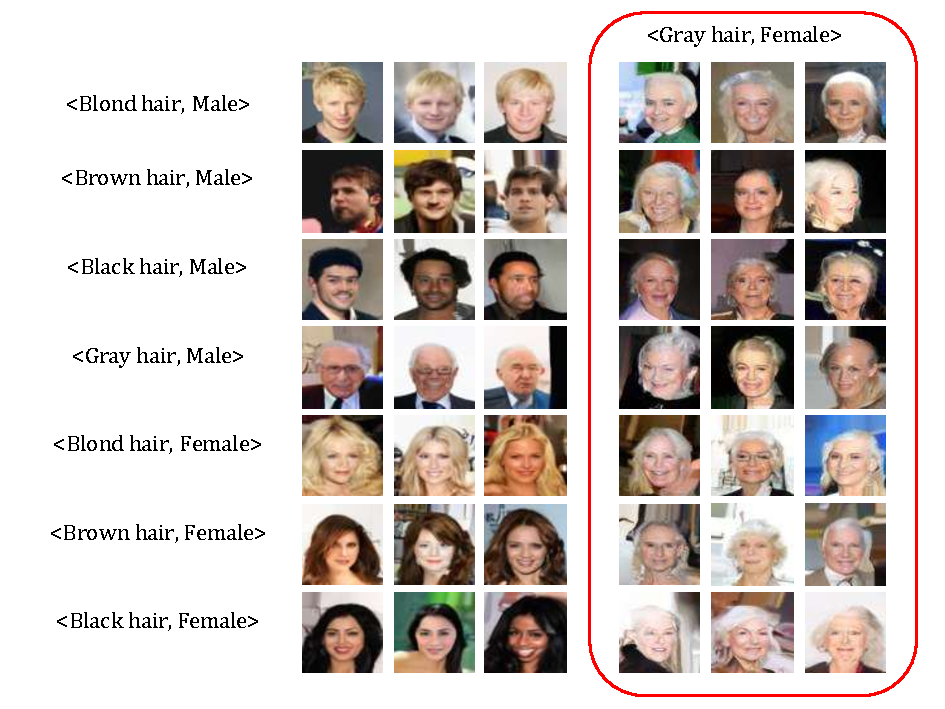
\includegraphics[width=1\linewidth]{figures/CelebA1.pdf}
    \caption{Under two condition setting of CelebA. Samples generated from CCDM, the unseen composition images are in red boxes.}
    \label{fig:sample_9}
\end{figure}

\begin{table} [H]
    \centering
    \begin{tabular}{cc}
         Classifier & Accuracy on validation set($\%$) $\uparrow$ \\
         \hline
         Gray hair classifier & 97.64 \\
         Female classifier & 99.12 \\
         
    \end{tabular}
    \caption{Accuracy of binary classifiers within image selector(Two conditions setting)}
    \label{CelebABinAcc}
\end{table}

\begin{table} [H]
    \centering
    \begin{tabular}{cccc}
         Architecture & $c_1$ accuracy $\uparrow$ & $c_2$ accuracy $\uparrow$ & All Corrects accuracy $\uparrow$ \\
         \hline
         Add  & 0.36 & 0.82 & 0.20\\
         AdaGN & \textbf{0.58} & 0.74 & \textbf{0.32}\\
         IC & 0.49 & 0.73 & 0.27 \\
         CA & 0.35 & \textbf{0.93} & 0.29 \\
    \end{tabular}
    \caption{Architecture comparison on CelebA Dataset (Two conditions setting)}
    \label{tab:CelebAAcc}
\end{table}

\begin{figure} [H]
    \centering
    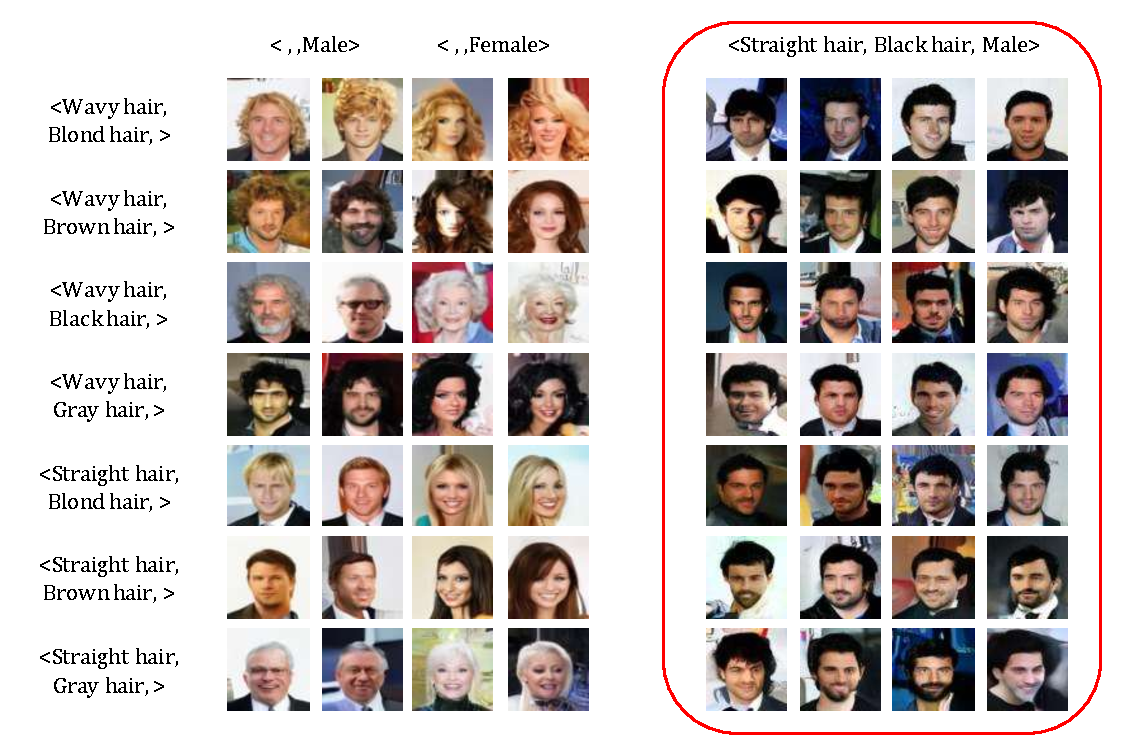
\includegraphics[width=1\linewidth]{figures/CelebA2.pdf}
    \caption{Under three condition setting of CelebA. Samples generated from CCDM, the unseen composition images are in red boxes.}
    \label{fig:sample_11}
\end{figure}

\begin{table} [H]
    \centering
    \begin{tabular}{cc}
         Classifier & Accuracy on validation set($\%$) $\uparrow$ \\
         \hline
         Straight hair classifier & 81.30 \\
         Black hair classifier & 100 \\
         Male classifier & 99.67 \\
    \end{tabular}
    \caption{Accuracy of binary classifiers within image selector(Three conditions setting)}
    \label{CelebABinAccTri}
\end{table}

\begin{table} [H]
    \centering
    \begin{tabular}{ccccc}
         Architecture & $c_1$ accuracy $\uparrow$ & $c_2$ accuracy $\uparrow$ & $c_3$ accuracy $\uparrow$ & All Corrects accuracy $\uparrow$ \\
         \hline
         Add  & \textbf{0.20} & 0.99 & 0.99 & \textbf{0.20}\\
         AdaGN & 0.11 & \textbf{1.0} & \textbf{1.0} & 0.11\\
         IC & \textbf{0.20} & 0.99 & \textbf{1.0} & 0.19\\
         CA & 0.06 & \textbf{1.0} & \textbf{1.0} & 0.06\\
    \end{tabular}
    \caption{Architecture comparison on CelebA Dataset (Three conditions setting)}
    \label{tab:CelebATriAcc}
\end{table}

In figure \ref{fig:sample_9} and figure \ref{fig:sample_11}, CCDM performs well on the CelebA dataset under the two-condition setting and three condition setting. However, the results generated by CCDM are not perfect. In table \ref{tab:CelebAAcc} and table \ref{tab:CelebATriAcc}, we compare the accuracy of generating unseen composition images using four different architectures. Although all can generate the unseen composition images correctly, the accuracy is not ideal. In the two-condition setting, where $c_1$ represents "Gray hair," this attribute has only a few samples in the dataset. In the three-condition setting $c_1$ represents "Straight hair", distinguishing between "Straight hair" and "Wavy hair" in male hair has low separability. We believe these factors contribute to the relatively low accuracy of CCDM in generating unseen composition images.

\section{Experiment analysis}
\begin{table} [H]
    \centering
    \begin{tabular}{cc}
         Architecture & Accuracy $\uparrow$\\
         \hline
         Add & 0.34\\
         AdaGN & 0.34\\
         IC & \textbf{0.42}\\
         CA & 0.36\\
    \end{tabular}
    \caption{Overall architecture comparison}
    \label{tab:OverallAcc}
\end{table}

Table \ref{tab:OverallAcc}  illustrates that among the four conditioning modules we used, Image Class Concatenation performs the best for compositional zero-shot image generation. This closely aligns with our expectations. For the diffusion model with compositional class labels as conditions, element-wise addition in the Addition module may aggregate information from multiple class labels, potentially hindering the model's ability to generate correct samples. The same rationale applies to AdaGN. Cross attention, when using compositional class label embeddings as keys and values, suffers from limited dimensions in both keys and values. Combined with the relatively insufficient data, it fails to fully exploit the power of cross attention. Concatenation, on the other hand, maximally preserves the information from compositional class embeddings. Additionally, concatenation avoids mixing the class embeddings of different conditions using addition, making it less prone to confusion for the model.


CCDM can achieve compositional zero-shot image generation across various datasets using the four architectures we employed. However, the quality of generated images is not consistently stable. We attribute this to not having found the most suitable conditioning module for compositional class labels yet. Nonetheless, the success on these datasets gives us confidence in using compositional class labels to guide the diffusion model. In future research, we aim to identify the optimal conditioning module for compositional class labels.

\chapter{Conclusion}
\label{chapter:conclusion}
We proposed a diffusion model conditioned on compositional class labels for compositional zero-shot image generation.Starting from the most basic dataset, we employed various methods to achieve Unseen data generation. Eventually, we adopted the approach of using compositional class labels as conditions to guide the generation model. By succeeding with the simplest dataset, we further validated that our model can achieve compositional zero-shot image generation through different datasets. Applying compositional cognitive abilities to the domain of image generation, our model can achieve "learning from old compositional concepts and generalizing to new compositional concepts."



%-------------------------------------------------------------------------------
% 參考文獻
%-------------------------------------------------------------------------------

% Set bib style
\bibliographystyle{IEEEtran}

% Add Bibliography to "Table of Contents"
\addBibToContents

% Usage:
%   \bibliography{bib/bib1,bib/bib2,...,bib/bibN} % 注意: 不要有空格
%
% For IEEEtran users:
%   DO NOT remove bib/BSTcontrol.bib when using IEEEtran.bst. The reason is that
% when we cite two papers of the same (or similar) authors, IEEEtran.bst would
% replace the author names with "------". To avoid this, we use BSTControl.bib
% to set ctldash_repeated_names to 'no'.
%
% For non IEEEtran users:
%   Please delete bib/ieeeBSTcontrol from \bibliography{}
\bibliography{bib/ieeeBSTcontrol,bib/thesis}

%-------------------------------------------------------------------------------
% 附錄
%-------------------------------------------------------------------------------

% Start appendix
% \appendix

% Add appendicies to "Table of Contents"
% \addAppxToContents

% 請從此開始依序擺放附錄
% %\chapter{附錄標題}

%\section{Testing}


%-------------------------------------------------------------------------------
% 作者簡歷
%-------------------------------------------------------------------------------

% 簡歷 (Only shown in a PhD dissertation)
\begin{vita}%

{\bf Harry Potter} is a character in TJ. K. Rowling's magic wonderland, ``Harry Potter." His research interests are finding the ways to trigger the catastrophe in Hogwarts.

\end{vita}

% 著作列表 (Only shown in a PhD dissertation)
\begin{publications}%

%%%%%%%%%%%%%%%%%%%%%%%%%%%%%%%%%%%%%%%%%%%%%%%%%%%%%%%%%%%%%%%%%%%%%%%%%%%%%%%

\section*{Journal Papers}
\begin{spacing}{1}
\begin{enumerate}

\item {\bf \underline{Harry Potter}}, Albus Dumbledore, ``The way to beat the dark lord, from Love to Horcrux," \textit{Journal of Supplementary}, vol. 777, no. 1, pp. 11--21, 2021

\end{enumerate}
\end{spacing}

%%%%%%%%%%%%%%%%%%%%%%%%%%%%%%%%%%%%%%%%%%%%%%%%%%%%%%%%%%%%%%%%%%%%%%%%%%%%%%%

\section*{Conference Papers}
\begin{spacing}{1}
\begin{enumerate}

\item {\bf \underline{害你駁倒}}, ``校園毀滅計畫," in \textit{International Conference of School Refresh}, 2021, Hogwarts, England

\end{enumerate}
\end{spacing}

%%%%%%%%%%%%%%%%%%%%%%%%%%%%%%%%%%%%%%%%%%%%%%%%%%%%%%%%%%%%%%%%%%%%%%%%%%%%%%%

\end{publications}

\end{document}